% STATUS: reviewed
\chapter{Konsolė ir viešoji svetainė}\label{ch:console}

Šiame skyriuje sistema rodoma iš ekrano pusės. Pradedama nuo dviejų žiniatinklio programų,
kurios dalijasi produkto adresu, --- viešosios svetainės, kuri paaiškina, kas yra produktas, ir
konsolės, kurioje atliekamas darbas, --- ir nuo rėmo, kuriame rodomas kiekvienas konsolės
puslapis: prisijungimo, navigacijos, dviejų kalbų, taip pat to, kaip puslapis įkelia savo
duomenis, seka vykdomą užduotį ir praneša apie klaidą. Toliau konsolė apeinama puslapis po
puslapio ta tvarka, kuria su puslapiais susiduria žmogus, ir prie kiekvieno nurodomas skyrius,
aiškinantis už jo slypintį mechanizmą. Vietos, kuriose konsolė prašo žmogaus apsispręsti,
surinktos į vieną lentelę. Skyrių užbaigia viešoji svetainė ir trumpas pasakojimas apie tai,
kaip konsolė sukurta.

Ekrano nuotraukos padarytos su konsolės testiniais duomenimis: visos juose matomos įmonės,
žmonės, datos, sumos ir modelių pavadinimai yra išgalvoti, ir nė vienas iš jų nepriklauso veikiančiai
sistemai. Dauguma nuotraukų yra anglų kalba; pirmoji konsolės kalba yra lietuvių, ir viena
nuotrauka ją ir rodo.

\begin{notebox}{Konsolė modelių nekviečia}
Nė viena iš dviejų programų nekviečia kalbos modelio. Konsolė siunčia užklausas API (Django) ir
asistento paslaugai, o kiekvieną modelio iškvietimą atlieka asistento paslauga (\cref{ch:arch}).
Konsolė leidžia žmogui iškvietimą pradėti --- išsiųsti pokalbio žinutę, pradėti analizę,
išbandyti instrukciją, --- o paskui parodo, kas grįžo, pažymi, ką parašė modelis, ir pasiūlo
vietą, kurioje sprendžia žmogus. Šių iškvietimų kelio kortelės pateiktos skyriuose, kuriems jie
priklauso; \cref{tab:console:modelbuttons} išvardija valdiklius, kurie iškvietimą pradeda.
\end{notebox}

% ------------------------------------------------------------
\section{Dvi programos viename šaltinyje}\label{sec:console:origin}

Vienas šaltinis (angl. \en{origin}) aptarnauja dvi vieno puslapio programas,
sukurtas iš vieno Vite projekto kataloge \file{vite/app/}. \term{Viešajai svetainei} priklauso
adreso šaknis (\code{/}): ji lankytojui be paskyros paaiškina, kas yra produktas.
\term{Konsolė} gyvena po \code{/console}: tai pati programa, pasiekiama prisijungus. Kiekviena
turi savo maršrutizatorių (\file{paths.js}), o nuoroda iš vienos į kitą yra paprasta nuoroda,
įkelianti kitą programą. Abi pradedamos iš vieno puslapio: žiniatinklio serveris konsolės atvaizde
(\file{vite/Caddyfile}) į kiekvieną adresą atsako failu \file{vite/app/index.html}, o vienintelis
šio puslapio scenarijus (\file{main.jsx}) adresui po \code{/console} paleidžia konsolę, bet kuriam
kitam --- viešąją svetainę ir atsisiunčia tik tą, kurią paleidžia.

\begin{figure}[H]
\centering
\begin{tikzpicture}
  \node[ext] (browser) at (0,0) {naršyklė};
  \node[svc, text width=24mm] (caddy) at (2.9,0) {statinis serveris\\\scriptsize\code{legalops-vite}};
  \node[svc, text width=30mm] (site) at (6.9,1.3) {viešoji svetainė\\\scriptsize\code{/} → \file{site/main.jsx}};
  \node[svc, text width=30mm] (console) at (6.9,-1.3) {konsolė\\\scriptsize\code{/console/*} → \file{console.jsx}};
  \node[chk, text width=30mm] (shared) at (11.6,1.3) {bendra: \file{brand.js}, \file{globals.css}, šriftai, vertimai, slapukas \code{locale}};
  \node[svc, text width=27mm] (api) at (11.6,-0.75) {API (Django)\\\scriptsize\code{/api/*}};
  \node[svc, text width=27mm] (asst) at (11.6,-2.15) {asistento paslauga\\\scriptsize\code{/api/assistant/chat}};
  \draw[flow] (browser) -- (caddy);
  \draw[flow] (caddy.north) |- (site.west);
  \draw[flow] (caddy.south) |- (console.west);
  \draw[call] (console.east) -- ++(4mm,0) |- (api.west);
  \draw[call] (console.east) -- ++(4mm,0) |- (asst.west);
  \draw[opt] (site.east) -- (shared.west);
  \draw[opt] (console.north east) -- (shared.south west);
  \node[note, below=0.5mm of site] {serverio nieko neprašo};
\end{tikzpicture}
\caption{Vienas šaltinis, dvi programos. Viešoji svetainė ir konsolė pradedamos iš to paties
puslapio, bet yra atskiros programos su atskirais maršrutizatoriais; su serverio puse kalbasi tik
konsolė. Bendra joms
išvaizda ir žodžiai: prekės ženklo spalvos ir šriftai, stilių failas, vertimai ir slapukas,
kuris įsimena kalbą.}\label{fig:console:origin}
\end{figure}

\paragraph{Kodėl dvi programos.} Viešoji svetainė skirta lankytojui, kuris neturi paskyros ir
galbūt niekada neprisijungs. Jos paleidimo modulis (\file{site/main.jsx}) neįkelia nei komponentų
bibliotekos, nei užklausų kliento, nei sesijos ir nieko neprašo iš serverio, todėl toks lankytojas
niekada neatsisiunčia konsolės. Konsolei visa tai reikalinga. Atskyrus abi programas, viešoji
svetainė lieka maža ir paprasta, o konsolė neša veikiančios programos svorį.

\paragraph{Kas joms bendra.} Prekės ženklo spalvos ir šriftai yra viena lentelė,
\file{brand.js}: paletė pagal pavadinimus (\code{COLORS}), du šriftų rinkiniai (\code{FONTS}) ir
keturių vertinimo tonų atspalviai (\code{TONES}), be jokios komponentų bibliotekos. Konsolė iš
šios lentelės kuria savo temą (\file{theme.js}); viešoji svetainė tas pačias reikšmes įrašo
puslapyje kaip CSS kintamuosius (\file{site/main.jsx}). Kadangi lentelė viena, abiejų pusių
spalvos negali išsiskirti. Joms taip pat bendri stilių failas (\file{globals.css}), du pačių
talpinami šriftai, žinučių failai ir slapukas \code{locale}, todėl lankytojas, svetainėje
pasirinkęs anglų kalbą, ir konsolę randa angliškai.

\paragraph{Seni adresai.} Kol šaknies neužėmė viešoji svetainė, ten gyveno konsolė. Iš to laiko
išsaugota nuoroda į ataskaitą ar pokalbį dabar patenka į svetainės maršrutizatorių, kurio
visa sugaunantis puslapis (\file{site/pages/Missing.jsx}) atpažįsta seną pirmąjį konsolės kelio
segmentą (\file{site/sitemap.js}) ir pakeičia adresą tuo pačiu po \code{/console}, išlaikydamas
užklausos dalį ir fragmentą. Bet kuris kitas nežinomas adresas gauna svetainės pranešimą
\enquote{Tokio puslapio nėra}.

% ------------------------------------------------------------
\section{Konsolės rėmas}\label{sec:console:frame}

Kiekvienas konsolės puslapis atvaizduojamas tame pačiame rėme (\file{components/layout/PageLayout.jsx}):
viršuje tamsi juosta, kairėje navigacija, puslapis su savo pavadinimo eilute, o pabaigoje
autorių teisių juosta. Šiame poskyryje aprašoma, ką šis rėmas atlieka kiekvienam puslapiui.

\subsection{Prisijungimas ir sesija}\label{sec:console:session}

\begin{figure}[htbp]
\centering
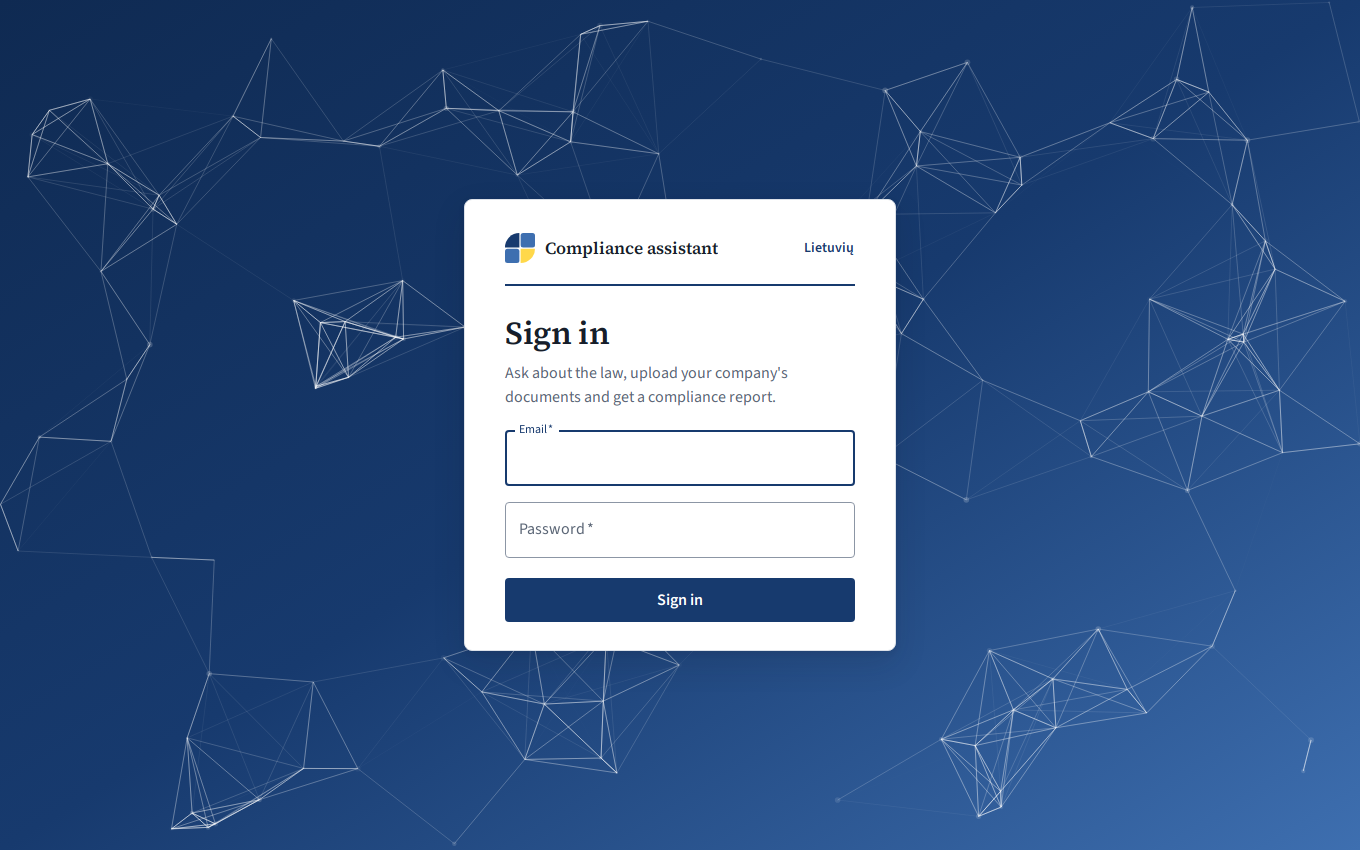
\includegraphics[width=.42\textwidth, trim=440 190 440 190, clip]{figures/screens/login}
\caption{Prisijungimo puslapis (\code{/console/login}). Žodinis ženklas lape veda į viešąją
svetainę; šalia jo yra kalbos jungiklis. Paskyras kuria administratorius, todėl registracijos
puslapyje nėra.}\label{fig:console:login}
\end{figure}

Prisijungimo puslapis (\file{pages/Login/Login.jsx}, \cref{fig:console:login}) prašo el. pašto
adreso ir slaptažodžio ir siunčia juos į \route{POST}{/api/auth/login}. Atsakymas yra
nepermatomas prieigos raktas, kurį konsolė laiko viename naršyklės vietinės saugyklos rakte
(\code{complianceToken}, \file{auth/token.js}) ir prideda prie kiekvienos vėlesnės užklausos
(\file{api/client.js}). Prieigos raktas sąmoningai išlieka perkrovus puslapį; serveris sesiją
vis tiek baigia po 30 dienų. Pats prisijungimas naudoja paprastą užklausą, o ne bendrą klientą,
nes neteisingas slaptažodis grąžina 401 ir neturi sukelti kliento nukreipimo \enquote{sesija
baigėsi}.

Paleista konsolė vieną kartą patikrina sesiją (\route{GET}{/api/auth/me}, \file{AuthGuard.jsx})
ir skiria keturias baigtis:

\begin{itemize}
  \item prieigos rakto nėra visai: iškart į prisijungimo puslapį, be užklausos;
  \item 401 į šią ar bet kurią vėlesnę užklausą: prieigos raktas išmetamas, o puslapis
    pakeičiamas adresu \code{/console/login?next=<here>&expired=1}, kuris rodo \ui{Sesija
    baigėsi\ldots} ir, prisijungus, grąžina naudotoją ten, kur jis buvo;
  \item serverio klaida ar neveikiantis tinklas: prieigos raktas lieka, o viso puslapio kortelė
    siūlo bandyti dar kartą --- serverio pusės paleidimas iš naujo neturi atjungti visų;
  \item atsakymas, kuris nėra paskyra (tuščias turinys, puslapis iš klaidingai nukreipiančio
    tarpinio serverio): ta pati kortelė; konsolė niekada neveikia prisijungusi kaip niekas.
\end{itemize}

Grįžimo kelias \code{?next=} paisomas tik tada, kai tai kelias tame pačiame šaltinyje
(\file{auth/session.js}, \code{safeNext}), todėl parametru negalima nusiųsti naudotojo į kitą
svetainę. Paskyros meniu tamsioje juostoje turi \ui{Paskyra} ir \ui{Atsijungti}; atsijungiant
serverio prašoma baigti sesiją, o prieigos raktas išmetamas bet kuriuo atveju.

\subsection{Navigacija ir ką mato kiekviena rolė}\label{sec:console:nav}

Navigacija (\file{components/layout/Sidebar.jsx}) grupuoja puslapius po penkiomis antraštėmis.
\Cref{tab:console:nav} pateikia jas su lietuviškomis etiketėmis, šalia --- angliškas, ir rolę,
kuri jas mato. Naudotojas turi vieną iš dviejų rolių: \code{user} arba \code{admin}.
Administratoriams skirtas punktas paprastam naudotojui paslepiamas, o pats maršrutas taip pat
saugomas: paprastas naudotojas, įvedęs tokį adresą, įprastame rėme gauna \enquote{Prieiga
ribojama} (\file{PageWrapper.jsx}). Ši patikra yra mandagumo gestas, o ne tikroji apsauga: API
paprastam naudotojui duomenų neduoda, kad ir ką rodytų konsolė (\cref{ch:security}).

\begin{table}[H]
\caption{Konsolės navigacija. Keliai pateikti be bazės \code{/console}.}\label{tab:console:nav}
\begin{tabularx}{\textwidth}{@{}L{25mm}L{40mm}L{33mm}Y@{}}
\toprule
\hd{Grupė} & \hd{Punktas (lietuviškai / angliškai)} & \hd{Kelias} & \hd{Kas mato} \\
\midrule
\ui{Pagrindinis} &\ui{Pokalbis} / Chat & \code{/}, \code{/chat/:threadId} & visi \\
 & \ui{Apžvalga} / Overview & \code{/dashboard} & visi \\
\ui{Atitiktis} &\ui{Įmonės} / Companies & \code{/companies}, \code{/companies/:companyId} & visi (savo įmones; administratorius mato visas) \\
 & \ui{Ataskaitos} / Reports & \code{/reports}, \code{/reports/:reportId} & visi (taip pat) \\
\ui{Teisė} &\ui{Teisės aktų bazė} / Legal corpus & \code{/corpus}, \code{/corpus/:documentId} & visi skaito; administratoriai ir keičia \\
 & \ui{Pareigų peržiūra} / Obligation review & \code{/obligations} & administratoriai \\
\ui{Administravimas} &\ui{DI instrukcijos} / AI prompts & \code{/prompts}, \code{/prompts/:slug} & administratoriai \\
 & \ui{MCP serveriai} / MCP servers & \code{/settings/mcp} & administratoriai \\
 & \ui{Naudotojai} / Users & \code{/users} & administratoriai \\
 & \ui{Veiksmų žurnalas} / Audit log & \code{/audit} & administratoriai \\
\ui{Sistema} &\ui{DI sąnaudos} / AI usage & \code{/usage} & visi (savo sąnaudas; administratorius mato visas) \\
 & \ui{Užduotys} / Jobs & \code{/jobs} & visi (savo užduotis; administratorius mato visas) \\
 & \ui{Paskyra} / Account & \code{/account} & visi \\
\bottomrule
\end{tabularx}
\end{table}

Dar du puslapiai pasiekiami ne iš navigacijos, o iš kitų puslapių: vieno atitikties programos
dokumento puslapis (\code{/programme/:productId}) ir prisijungimo puslapis. Navigacijos stulpelį
galima prisegti atvirą arba suskleisti į piktogramų juostelę, kuri atsiveria virš puslapio
užvedus žymeklį; pasirinkimas įsimenamas naršyklėje. Telefone navigacija yra stalčius,
atidaromas iš tamsios juostos.

\subsection{Dvi kalbos}\label{sec:console:lang}

Konsolė kalba lietuviškai ir angliškai, pirmiausia lietuviškai: lietuvių kalba yra numatytoji ir
atsarginė (\file{i18n.jsx}, \code{DEFAULT_LOCALE = 'lt'}). Jungiklis tamsioje juostoje įvardija
kitą kalbą (\ui{English} lietuviškame puslapyje, \ui{Lietuvių} angliškame), iškart, be perkrovimo,
pakeičia visą sąsają ir metams įsimena pasirinkimą slapuke \code{locale}. Paskui jį seka puslapio
pavadinimas, dokumento kalba (\code{<html lang>}) ir komponentų bibliotekos įtaisyti tekstai.
Sąsajos kalba nėra turinio kalba: ataskaita ar programos dokumentas rašomas ta kalba, kuri
pasirinkta jį pradedant (numatytoji --- sąsajos kalba), o pokalbių asistentas atsako ta kalba,
kuria rašo naudotojas.

\subsection{Kaip puslapis įkelia duomenis ir seka užduotį}\label{sec:console:data}

Visos užklausos, išskyrus prisijungimą ir srautu siunčiamą pokalbio atsakymą, eina per vieną
klientą (\file{api/client.js}), o kiekvienas skaitymas --- per vieną TanStack Query podėlį,
sukurtą \file{main.jsx} su vienu pakartotiniu bandymu, todėl du kartus nepavykusi užklausa rodo
savo klaidą, o ne sukasi be galo. Puslapiai skaito; iš serverio niekas nestumiama. Ilgai
trunkantis darbas --- analizė, generavimas, teisės akto įkėlimas --- vykdomas kaip
\term{užduotis} užduočių vykdytoje (\cref{ch:arch}), o jį rodantis puslapis, kol darbas vyksta,
kas tam tikrą laiką klausia iš naujo, paskui liaujasi. \Cref{tab:console:polling} išvardija
intervalus.

\begin{table}[H]
\caption{Kur konsolė seka vykdomą darbą ir kaip dažnai klausia. Kiekviena apklausa liaujasi, kai
darbas baigiasi; ataskaita, laukianti apimties patvirtinimo, neapklausiama, nes ją pajudinti gali
tik žmogus.}\label{tab:console:polling}
\begin{tabularx}{\textwidth}{@{}L{48mm}Yr@{}}
\toprule
\hd{Puslapis} & \hd{Klausia, kol} & \hd{Dažnis} \\
\midrule
Viena ataskaita (\file{ReportDetail.jsx}) & analizė laukia eilėje arba vykdoma & 3 s \\
Jos eigos kortelė (\file{ReportProgress.jsx}) & kortelė rodoma (užduoties etapai) & 3 s \\
Ataskaitų sąrašas, įmonės ataskaitų skiltis & kuri nors analizė laukia eilėje arba vykdoma & 5 s \\
Programos dokumento puslapis & generavimas laukia eilėje arba vykdomas & 3 s \\
Įmonės programos skiltis & kuris nors programos dokumentas laukia eilėje arba generuojamas & 5 s \\
Vienas teisės aktų bazės aktas & jo paskutinė užduotis (arba vertintojo užduotis) laukia eilėje arba vykdoma & 3 s \\
Teisės aktų katalogas & kuris nors aktas dar įkeliamas & 5 s \\
Įmonės dokumentų skiltis & per paskutines 10 minučių įkeltas dokumentas laukia savo indekso & 5 s \\
Pokalbio kortelės (ataskaita, programos dokumentas) & vykdoma analizė arba generavimas & 5 s \\
Apžvalga & visada (užduočių eilė); ataskaitos, kol kuri nors vykdoma & 10 s \\
Užduotys (\code{LIVE_MS}, \code{IDLE_MS}) & kas nors laukia eilėje arba vykdoma; kitaip & 2 s; 30 s \\
\bottomrule
\end{tabularx}
\end{table}

Užduočių vykdytojas eigą rašo angliškai (\enquote{3/10 batches}); konsolė išverčia žinomus
pranešimus ir užduoties objektą (\code{report:<id>}, \code{corpus:<id>}, \code{product:<id>})
paverčia etikete su nuoroda į jo puslapį (\file{hooks/useJobText.js}), kad į ekraną nepatektų
nieko, kas skirta mašinai.

Tai, ką žmogus nori vėl rasti, gyvena puslapio adrese: skiltis, filtrai, paieška, lentelės
puslapis ir rikiavimas (\file{hooks/useViewParams.js}). Pakeitimas pakeičia istorijos įrašą,
o ne prideda naują, todėl mygtukas \enquote{Atgal} išveda iš puslapio, užuot atšaukęs filtrą, o
nukopijuotas adresas kolegai atveria tą patį vaizdą; išsamaus puslapio grįžimo nuoroda grąžina
į sąrašą tokį, koks jis buvo paliktas (\file{utils/navigationMemory.js}). Forma su
neišsaugotais pakeitimais prieš paliekant puslapį paklausia.

\subsection{Klaidos ir tušti sąrašai}\label{sec:console:errors}

Nepavykęs skaitymas niekada neatrodo kaip tuščias sąrašas. Kiekviena puslapio dalis turi savo
užklausą ir, jai nepavykus, vietoj duomenų rodo raudoną langelį su priežastimi ir galimybe
bandyti dar kartą (\file{components/ErrorState/ErrorState.jsx}); viena nepavykusi dalis kitų
nenuverčia. Įkeltas, bet tuščias sąrašas rodo piktogramą, sakinį ir, jei toks yra, kelią
toliau (\file{components/EmptyState/EmptyState.jsx}). Nepavykęs pakeitimas (bet kas, išskyrus
skaitymą) ekrano viršuje parodo trumpą pranešimą; dialogo langas savo atsisakymą rodo savo viduje.

API į nesėkmę atsako angliškai parašytu sakiniu ir kodu. Lietuviška sąsaja niekada neturi rodyti
angliško sakinio ar neapdoroto kodo, todėl kiekviena nesėkmė susiejama su pranešimu
(\file{utils/errors.js}): žinomas kodas --- su savo išverstu sakiniu, kitaip HTTP būsena --- su
sakiniu, kitaip --- tinklo ar laiko limito sakinys. Užklausų dažnio ribojimo pranešimas nurodo,
kiek laukti, jei serveris tai pasakė. Puslapis, kurio kodo dalies nepavyksta įkelti (naršyklės
skirtukas, senesnis už paskutinį diegimą), vieną kartą persikrauna pats; tik antra nesėkmė
parodo kortelę, kad programa buvo atnaujinta (\file{pages/RouteError/RouteError.jsx}).

% ------------------------------------------------------------
\section{Konsolė puslapis po puslapio}\label{sec:console:tour}

Puslapiai eina ta tvarka, kuria su jais susiduria žmogus: prisijungus --- pokalbis, apžvalga,
įmonės ir jų dokumentai, ataskaitos, tai, kas lieka po ataskaitos, atitikties programa ir jos dokumentai,
o paskui administratoriaus puslapiai.

\subsection{Pokalbis}\label{sec:console:chat}

\begin{figure}[htbp]
\centering
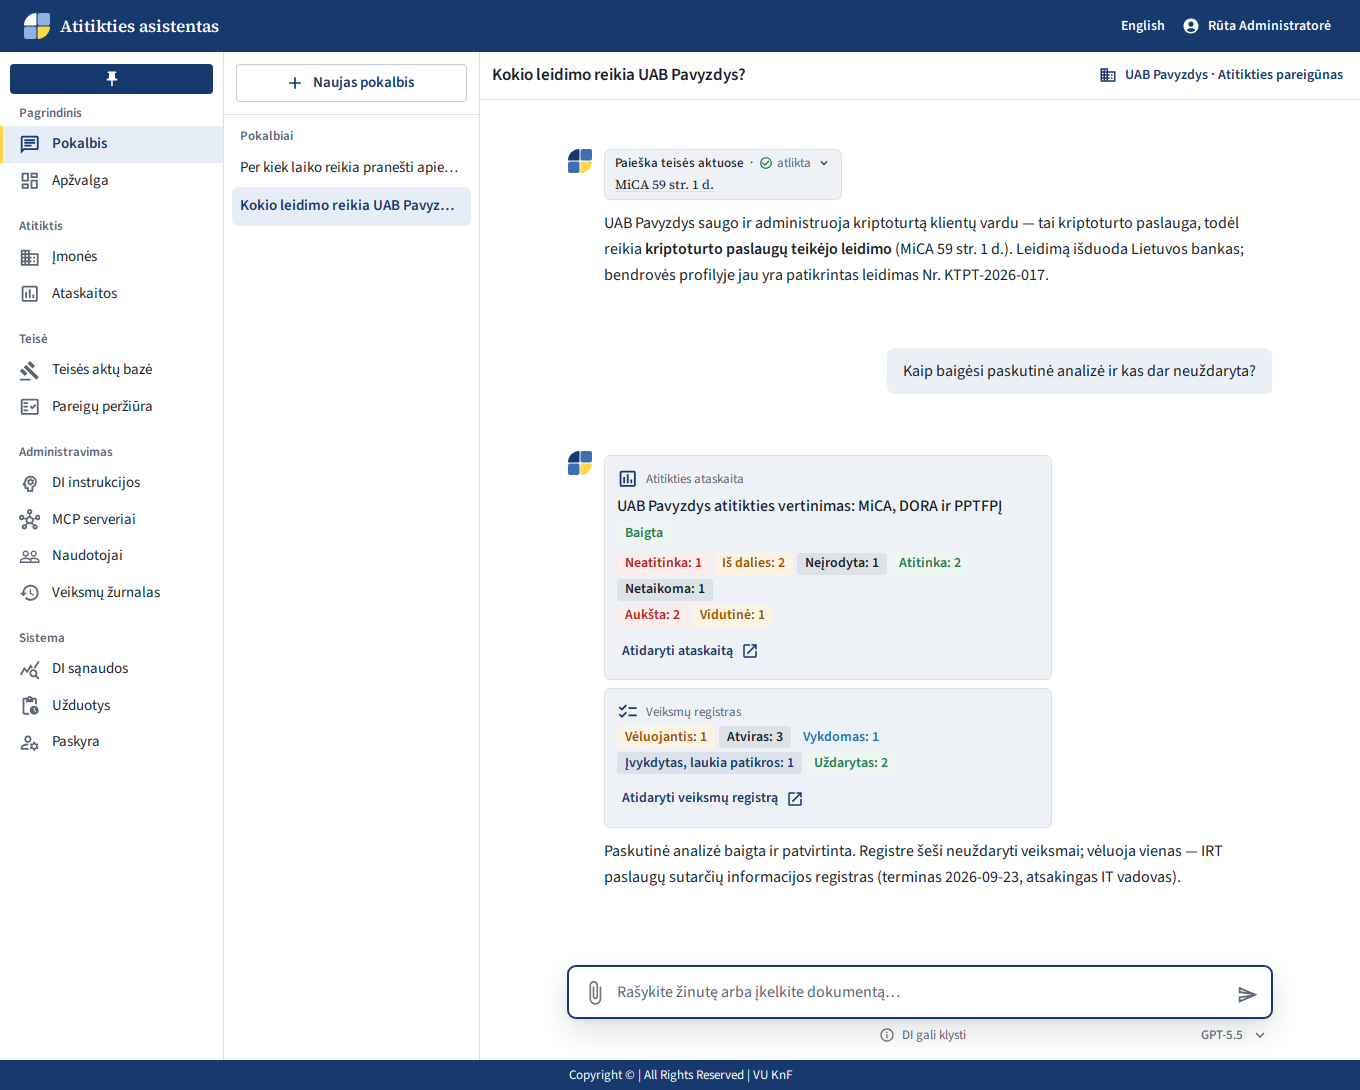
\includegraphics[width=.86\textwidth]{figures/screens/chat-tools-lt}
\caption{Pokalbis lietuviškai, kaip jį mato administratorius (\code{/console/chat/:threadId}).
Kairėje navigacija ir pokalbių sąrašas; atsakyme --- įrankio žymelė (\ui{Paieška teisės aktuose
· atlikta}) su perskaityta nuostata ir dvi įrankių kortelės: ataskaita su skaičiais ir veiksmų
registras. Antraštėje --- susieta įmonė ir rolė; po rašymo lauku --- pranešimas \ui{DI gali
klysti} ir pokalbio modelis.}\label{fig:console:chat}
\end{figure}

Pokalbis yra pirmasis konsolės puslapis (\file{pages/Chat/Chat.jsx}, \cref{fig:console:chat}).
Jį sudaro trys dalys: pokalbių sąrašas, pokalbio eiga ir įmonės skydelis.

\paragraph{Pokalbiai.} Sąraše po \ui{Naujas pokalbis} surašyti naudotojo pokalbiai. Pokalbio
pavadinimą iš pirmosios žinutės sudaro nedidelis modelis (\prompt{chat.title}); pavadinimas,
kurį naudotojas suteikia pieštuku savo eilutėje, niekada nepakeičiamas. Šiukšliadėžės piktograma,
paprašiusi patvirtinimo, pašalina pokalbį iš sąrašo; serveris jį laiko archyve. Grįžus į
pokalbį iš kito puslapio, atsiveria paskutinis pokalbis; pokalbio nuoroda pačiame pokalbyje
pradeda naują.

\paragraph{Pokalbio eiga.} Žinutė siunčiama paspaudus Enter (Shift+Enter perkelia eilutę).
Atsakymą rašo asistento paslauga, jis srautu siunčiamas iš \route{POST}{/api/assistant/chat};
jis rašomas serveryje, todėl uždarius puslapį neprarandamas, o bandant palikti puslapį, kol jis
rašomas, pirmiausia paklausiama. \ui{Stabdyti atsakymą} jį sustabdo ir išsaugo tai, kas jau
parašyta. Atsakymą galima nukopijuoti arba sugeneruoti iš naujo, žinutę --- pataisyti.
Atsakymai yra modelio parašytas Markdown tekstas ir eina per vieną saugų atvaizdavimo komponentą
(\file{components/Markdown/Markdown.jsx}): išlieka tik žiniatinklio ir pašto nuorodos,
paveikslai virsta nuorodomis, neapdorotas HTML rodomas kaip tekstas.
Po lauku rodomas trumpas pranešimas \ui{DI gali klysti}, kurio piktograma atveria visą skaidrumo
tekstą, o dešinėje --- pokalbio modelis: DI tinklų sąsajos pokalbių modelių meniu su kainomis,
kad brangesnis modelis būtų sąmoningas pasirinkimas, mažinantis naudotojo dienos biudžetą
(\file{pages/Chat/ModelPicker.jsx}).

\paragraph{Įrankių kortelės.} Kai asistentas naudoja įrankį, atsakymas tai parodo ten, kur
įrankis buvo panaudotas (\file{pages/Chat/ToolCards.jsx}). Numatytasis vaizdas yra žymelė su
įrankio pavadinimu, jo būsena žodžiais ir piktograma (\ui{vykdoma…}, \ui{atlikta}, \ui{nepavyko},
\ui{nutraukta}), o ją atvėrus --- tiksli įvestis ir rezultatas; nepavykęs iškvietimas rodo savo
klaidos kodą. Kai kurie įrankiai turi savo kortelę: teisės aktų bazės paieška ar nuorodų patikra
išvardija perskaitytas nuostatas, kiekvieną su nuoroda į oficialų tekstą, o patikros atveju ---
pažymėtą jos verdiktu; kainos įvertis rodo viršutinę kainos ribą ir likusį biudžetą, kad
naudotojas galėtų atsakyti į asistento klausimą \enquote{ar pradėti?}; ataskaitos kortelė rodo
jos būseną, eigą realiuoju laiku ir skaičius su nuoroda į ataskaitą; programos dokumento ir
veiksmų registro kortelės tą patį daro savo objektams. Išorinio MCP serverio įrankis pažymimas
\ui{Išorinis šaltinis}. Patys įrankiai aprašyti priede (\cref{app:tools}); pokalbio mechanizmas ---
\cref{ch:chat}.

\paragraph{Failai.} Failas numetamas ant rašymo lauko, įklijuojamas arba pasirenkamas sąvaržėle.
Jis iškart įkeliamas į \route{POST}{/api/documents} ir tampa vienu iš naudotojo dokumentų;
žymelė ant žinutės rodo įkėlimo eigą, o paskui --- jo teksto būseną. Konsolė dar prieš
siųsdama atsisako tipo, kurio sistema negali perskaityti, arba didesnio nei 50~MB failo
(\code{MAX_DOCUMENT_BYTES}, \file{constants/uploads.js}, API ribos kopija) ir virš lauko
nurodo atmestą failą ir priežastį.

\paragraph{Įmonės skydelis.} Mygtukas pokalbio antraštėje įvardija pokalbio įmonę ir rolę ir
atveria įmonės skydelį (\file{pages/Chat/CompanyPanel.jsx}). Jo viršuje pokalbis susiejamas su
viena iš naudotojo įmonių (\ui{Susieta įmonė}) ir, jei norima, su vienu iš tos įmonės rolių
profilių, kad asistentas atsakytų iš tos rolės pozicijų. Žemiau pateikiami įmonės profilis, jos
licencijos ir sertifikatai (deklaruoti ar patikrinti), jos dokumentai su jų teksto būsena, jos
rolės ir nuoroda į visą įmonės puslapį. Skydelis perskaitomas iš naujo, kai baigiasi ėjimas,
nes asistentas savo įrankiais galėjo ką tik sukurti ar pakeisti įmonę.

\subsection{Apžvalga}\label{sec:console:overview}

\ui{Apžvalga} (\file{pages/Dashboard/Dashboard.jsx})
atsako į klausimą \enquote{kam reikia dėmesio}: skaičių eilutė (įmonės, baigtos ataskaitos,
vykdomos analizės kartu su laukiančiomis apimties patvirtinimo, parengti teisės aktai iš visų;
administratoriui dar peržiūros laukiančios pareigos ir naudotojai), šios dienos DI biudžetas kaip
matuoklis, naujausios ataskaitos ir įmonės, teisės aktų bazės būklė su aktais, kurių įkėlimas
nepavyko, ir užduočių eilė su laukiančių, vykdomų ir nepavykusių skaičiais, kurių kiekvienas yra
nuoroda į užduočių puslapį, atfiltruotą pagal tą būseną. Kiekviena kortelė įkeliama ir gali nepavykti
nepriklausomai nuo kitų.

\subsection{Įmonės}\label{sec:console:companies}

\ui{Įmonės} (\file{pages/Companies/Companies.jsx}) išvardija naudotojo įmones; administratorius
mato visų įmones su savininko vardu ir gali apsiriboti savosiomis mygtuku \ui{Tik mano}. Paieška
vykdoma serveryje pagal pavadinimą ir registracijos kodą. \ui{Nauja įmonė} sukuria profilį su
pavadinimu, kodu, įstaigos tipu ir šalimi; visa kita pildoma įmonės puslapyje arba pokalbyje
per asistentą.

\begin{figure}[htbp]
\centering
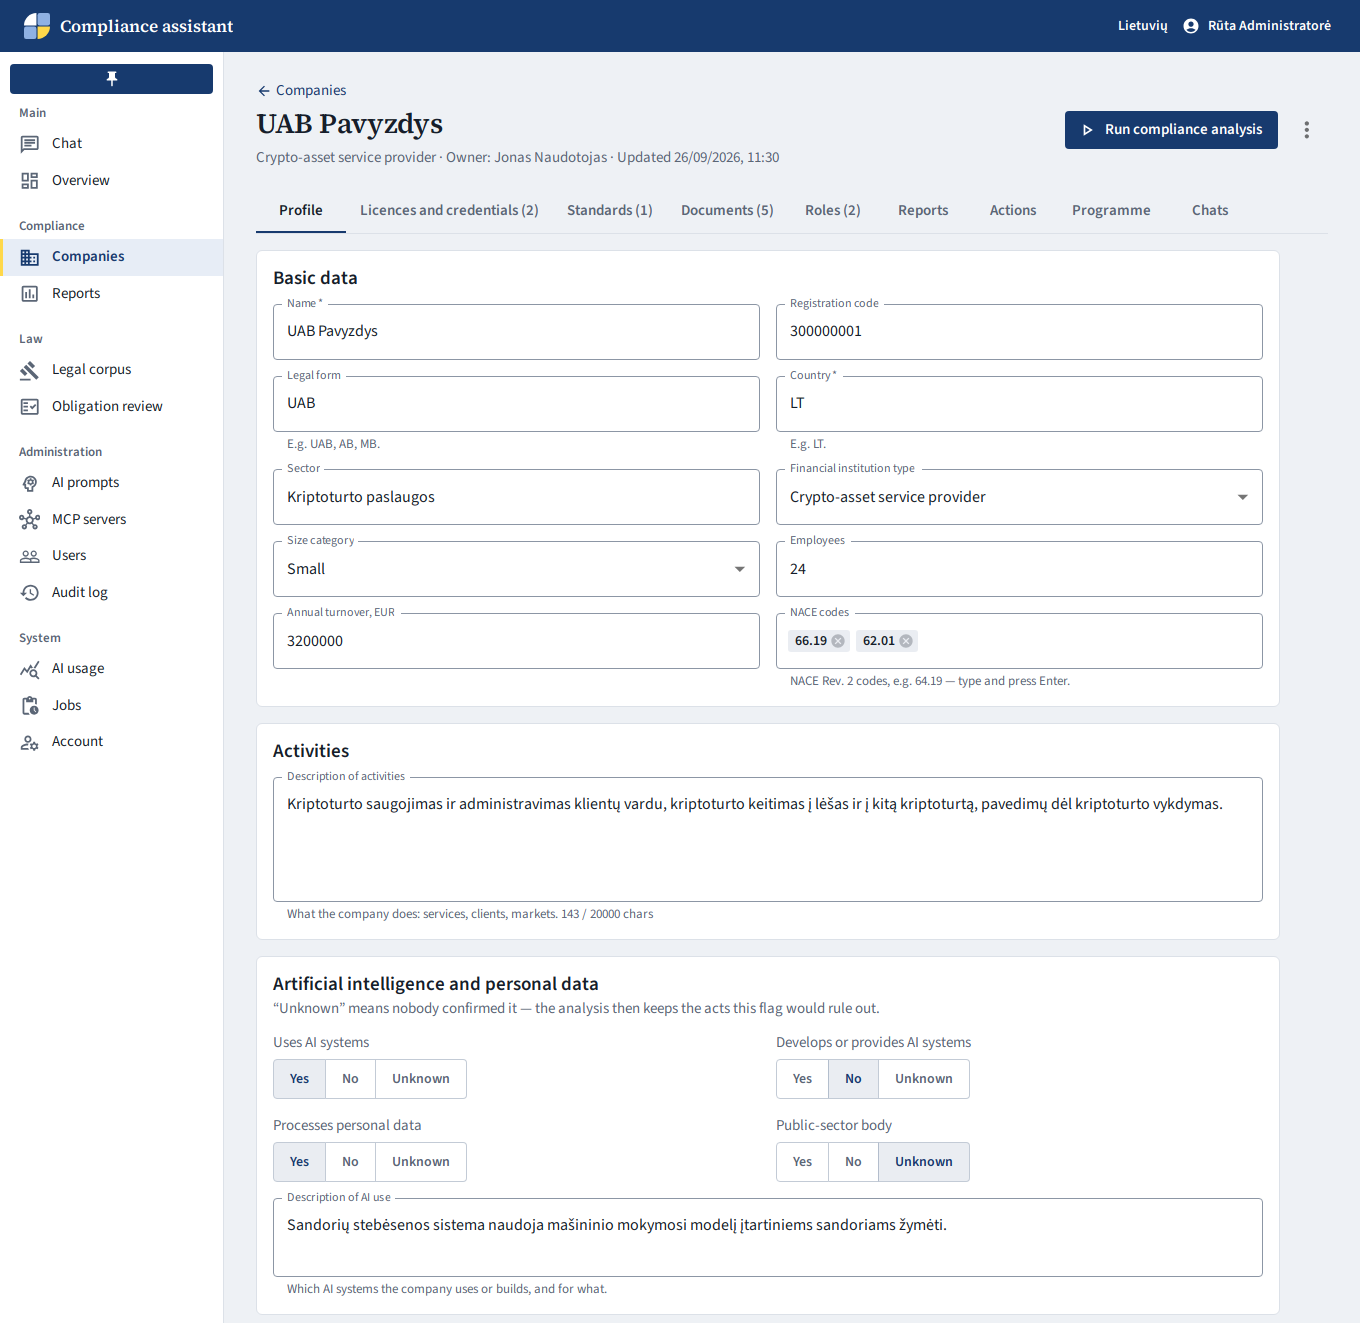
\includegraphics[width=.76\textwidth, trim=240 613 0 52, clip]{figures/screens/company-profile}
\caption{Įmonės puslapis, profilio skiltis (\code{/console/companies/:companyId}), viršutinė
dalis. Atkreipkite dėmesį į devynias skiltis su skaičiais pavadinimuose, \ui{Pradėti atitikties
analizę} antraštėje ir savininko vardą paantraštėje, kurį mato
administratorius.}\label{fig:console:company}
\end{figure}

Įmonės puslapis (\file{pages/Companies/CompanyDetail.jsx}, \cref{fig:console:company}) turi
devynias skiltis, išvardytas \cref{tab:console:companytabs}. Skiltis laikoma adrese
(\code{?tab=}), o kartą atverta skiltis lieka įkelta, todėl neišsaugoti profilio pakeitimai
išlieka pažvelgus į kitą skiltį. Antraštėje yra \ui{Pradėti atitikties analizę} ir meniu su
\ui{Naujas pokalbis apie įmonę} ir \ui{Ištrinti įmonę}; įmonės negalima ištrinti, kol vykdoma
kuri nors jos analizė. Telefono pločio ekrane devynių skilčių juosta slenka, o skiltis, atverta
tiesiogine nuoroda, gali atsidurti po slinkimo rodykle.

\begin{table}[H]
\caption{Devynios įmonės puslapio skiltys (\code{TABS} faile \file{CompanyDetail.jsx}), jų
tvarka.}\label{tab:console:companytabs}
\begin{tabularx}{\textwidth}{@{}L{38mm}YL{19mm}@{}}
\toprule
\hd{Skiltis} & \hd{Ką rodo ir ką gali daryti žmogus} & \hd{Mechanizmas} \\
\midrule
\ui{Profilis} & Visi profilio laukai kortelėse: pagrindiniai duomenys, veikla, DI ir asmens
duomenys, finansų rinkos klasifikacija (nustato asistentas, tik skaitymui), papildomi duomenys JSON
pavidalu. Keturi faktai --- naudoja DI, teikia DI, tvarko asmens duomenis, viešojo sektoriaus
subjektas --- yra taip / ne / nežinoma; \enquote{nežinoma} siunčiama kaip \code{null}, niekada
nespėjama, ir analizėje palieka aktus, kuriuos tas faktas atmestų. Išsaugoma viena užklausa,
kurioje tik pakeisti laukai. &
\cref{ch:company} \\
\ui{Leidimai ir licencijos} & Licencijos, leidimai, registracijos, sertifikatai, kiekvienas
\ui{Deklaruota} arba \ui{Patikrinta}. \ui{Pažymėti patikrintu} yra patvirtinamas veiksmas,
užrašantis, kas ir kada. &
\cref{ch:company} \\
\ui{Standartai} & Standartai, pagal kuriuos įmonė sertifikuota, kuriuos diegia ar planuoja,
pasirinkti iš teisės aktų bazės standartų; kiekviena vėlesnė analizė juos vertina. &
\cref{ch:company,ch:report} \\
\ui{Dokumentai} & Įkėlimo sritis (dokumento rūšis, numetimo zona), paieška dokumentų tekste ir
sąrašas su teksto ir indekso būsena bei inventoriaus santrauka. Eilutė atveria dokumento stalčių. &
\cref{ch:company} \\
\ui{Rolės} & Rolių profiliai, kuriuos gali perimti pokalbis: pavadinimas, ne ilgesnis nei
6\,000 simbolių rolės kontekstas ir jo šaltiniai įmonės dokumentuose. & \cref{ch:chat} \\
\ui{Ataskaitos} & Įmonės analizės, kaip ataskaitų puslapyje. & \cref{ch:report} \\
\ui{Veiksmai} & Veiksmų registras, o po juo --- teisės aktų pokyčiai
(\cref{sec:console:register}). & \cref{ch:register} \\
\ui{Programa} & Trys atitikties programos dokumentai (\cref{sec:console:programme}). &
\cref{ch:programme} \\
\ui{Pokalbiai} & Paties naudotojo pokalbiai apie šią įmonę, kiekvienas --- nuoroda į pokalbį. &
\cref{ch:chat} \\
\bottomrule
\end{tabularx}
\end{table}

\paragraph{Dokumentai ir dokumento stalčius.} Dokumentas įkeliamas dokumentų skiltyje: pirmiausia
pasirenkama rūšis (politika, procedūra, sutartis, registras, kita), paskui failai numetami arba
pasirenkami; kiekvienas keliamas su savo eigos juosta. Tekstas išgaunamas įkėlimo metu, o
indeksą vėliau sukuria užduočių vykdytojas, todėl sąrašas kurį laiką klausia iš naujo. Paieškos
laukas semantinę paiešką įmonės dokumentuose vykdo tik paspaudus Enter, nes kiekviena paieška
vektorizuoja užklausą ir šiek tiek kainuoja; rastas atitikmuo atveria dokumentą toje vietoje.

\file{pages/Companies/useDocumentIntake.js} --- kabliukas, kuriuo skiltis įkeltos partijos
dokumentus perduoda asistentui: atveria įmonės pokalbį
(\route{POST}{/api/chat/threads}) ir naudotojo vardu išsiunčia vieną ėjimą
(\route{POST}{/api/assistant/chat}) su prisegtais dokumentais, kurie turi tekstą, --- ne
daugiau kaip 29 vienam ėjimui, nes žinutėje telpa 30 dalių. Tai, kas įkeliama šiam ėjimui
vykstant, palaukia ir tada patenka į atskirą pokalbį, kad joks ėjimas nemokėtų už ankstesnių
dokumentų skaitymą dar kartą. Niekam nieko nereikia prašyti: pagal pirmąją pokalbio
instrukcijos taisyklę asistentas dokumentus perskaito ir įrašo tai, ką jie nustato, ---
profilį, kiekvieno dokumento rūšį, licencijas, standartus, rolių profilius (\cref{ch:chat}).
Pranešimas po įkėlimo zona pasako, kad asistentas skaito ir ką pildo, pateikia nuorodą į
pokalbį ir pasako, kuo ėjimas baigėsi: atlikta arba nebaigta, priežastį nurodant paties
pokalbio sakiniu (išnaudotas šios dienos biudžetas, asistentas nesukonfigūruotas, nutrūkęs
atsakymas). Ėjimo, kuris atmestas dar neprasidėjęs, pokalbyje nieko nėra, todėl jis vėl
archyvuojamas. Ėjimas vykdomas serveryje ir tęsiasi uždarius puslapį.

\begin{figure}[htbp]
\centering
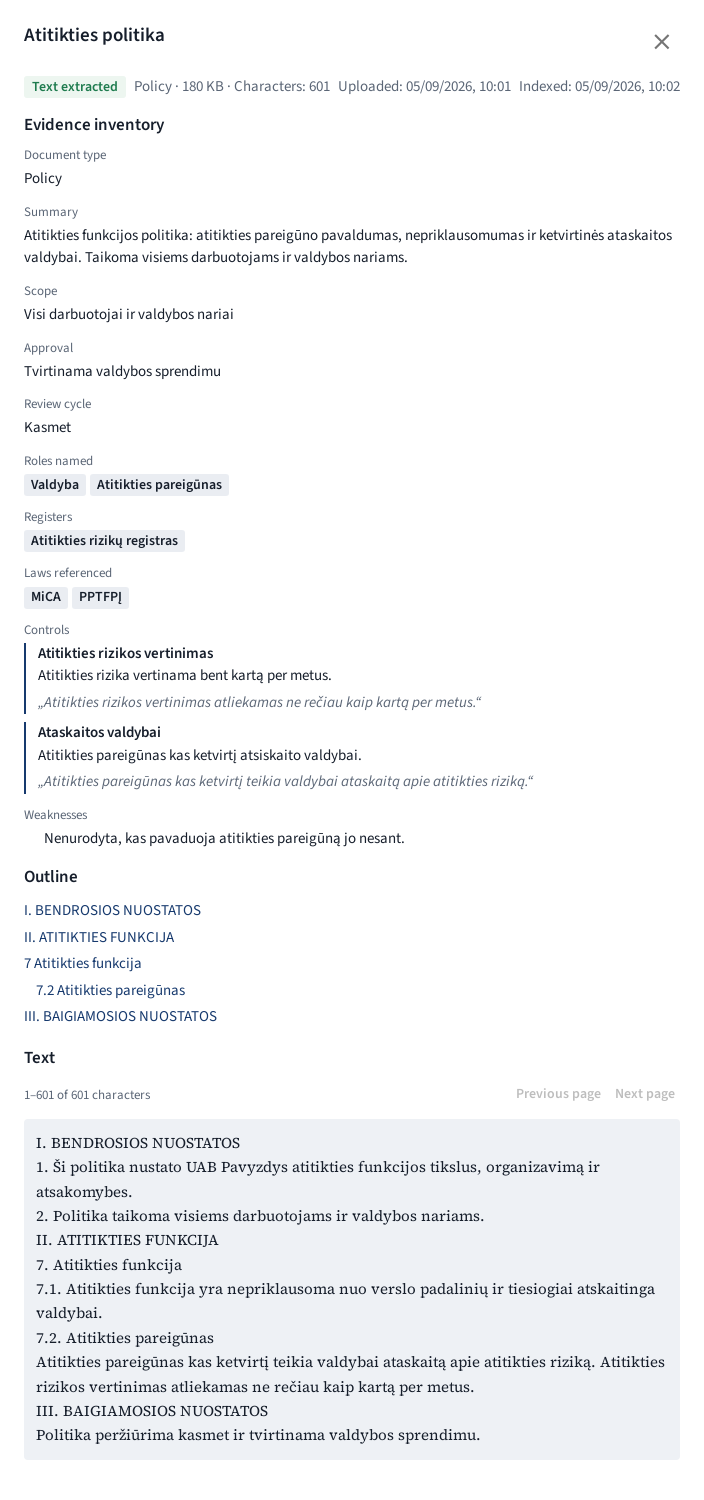
\includegraphics[width=.50\textwidth, trim=0 640 0 0, clip]{figures/screens/document-drawer}
\caption{Dokumento stalčiaus viršus: teksto būsena ir įrodymų inventorius, kurį modelis išskaitė
iš dokumento: kontrolės priemonės su citatomis, jame minimos rolės, registrai ir įstatymai,
jo silpnosios vietos. Žemiau eina turinys ir puslapiais suskirstytas
tekstas.}\label{fig:console:drawer}
\end{figure}

\term{Dokumento stalčius} (\file{pages/Companies/DocumentDrawer.jsx}, \cref{fig:console:drawer})
yra vienintelė vieta konsolėje, kur skaitomas įmonės dokumentas. Jis rodo dokumento inventorių
--- tai, ką analizė iš jo išskaitė, sukurta vieną kartą ir laikoma podėlyje (\cref{ch:company}),
--- jo turinį, kurio antraštės nušoka į savo vietą, ir jo tekstą 20\,000 simbolių langais
(\code{TEXT_WINDOW}). Stalčius taip pat yra ta vieta, į kurią veda išvados įrodymas: atvertas iš
citatos, jis rodo teksto puslapį, kuriame ji yra, o cituota ištrauka pažymėta geltonu
žymekliu, todėl skaitytojas gali matyti sakinį, kuriuo rėmėsi modelis, jo kontekste.

\subsection{Ataskaitos}\label{sec:console:reports}

\ui{Ataskaitos} (\file{pages/Reports/Reports.jsx}) išvardija naudotojo įmonių analizes
(administratoriaus --- visas), filtruojamas pagal įmonę ir būseną. Ataskaitos būsena yra viena
iš šių: \ui{Laukia eilėje}, \ui{Vykdoma}, \ui{Laukia apimties patvirtinimo}, \ui{Baigta},
\ui{Nepavyko} ir \ui{Atšaukta}. \ui{Nauja analizė} atveria pradžios dialogą su įmonės
pasirinkimu; iš įmonės puslapio įmonė jau nustatyta. Ką daro analizė, aprašyta \cref{ch:report};
čia --- ką iš jos mato žmogus.

\begin{figure}[H]
\centering
\begin{tikzpicture}[node distance=5mm and 7mm, every node/.append style={text width=27mm}]
  \node[man] (start) {pradžia\\\scriptsize sutikimas su įverčiu};
  \node[ai, right=of start] (p1) {vykdoma pirmoji dalis\\\scriptsize eigos kortelė};
  \node[man, right=of p1] (scope) {apimties peržiūra\\\scriptsize jungikliai, patvirtinimas};
  \node[ai, right=of scope] (p2) {vykdoma antroji dalis\\\scriptsize eigos kortelė};
  \node[svc, below=9mm of p2] (done) {baigta\\\scriptsize šešios skiltys, eksportas};
  \node[man, left=of done] (review) {išvadų peržiūra\\\scriptsize būsenos keitimas, priežastis};
  \node[man, left=of review] (sign) {patvirtinimas\\\scriptsize arba jo atšaukimas};
  \node[svc, left=of sign] (reg) {veiksmų registras\\\scriptsize į jį patenka planas};
  \draw[flow] (start) -- (p1);
  \draw[flow] (p1) -- (scope);
  \draw[flow] (scope) -- (p2);
  \draw[flow] (p2) -- (done);
  \draw[flow] (done) -- (review);
  \draw[flow] (review) -- (sign);
  \draw[flow] (sign) -- (reg);
  \draw[opt] (p1.north) -- ++(0,4mm) -| node[lbl, pos=.25]{be peržiūros} (p2.north);
\end{tikzpicture}
\actorlegend
\caption{Ataskaitos puslapis per visą jos gyvenimą, kaip jį rodo konsolė. Analizė sustoja po
pirmosios, pigios dalies ir laukia, kol žmogus patvirtins aktų sąrašą, nebent ji pradėta be
peržiūros (taškinė linija). Baigtą ataskaitą peržiūri ir patvirtina žmogus; patvirtinimas
pajudina įmonės veiksmų registrą. Modelio iškvietimai abiejose vykdomose dalyse aprašyti
\cref{ch:report}.}\label{fig:console:reportlife}
\end{figure}

\paragraph{Analizės pradžia.} Pradžios dialogas (\file{pages/Reports/StartAnalysisDialog.jsx},
\cref{fig:console:start}) prašo ataskaitos kalbos, neprivalomos apimties (\ui{Tik šie teisės
aktai (neprivaloma)}) ir dviejų parinkčių. \ui{Įvertinti ir įmonės vidaus reikalavimų
laikymąsi} prideda patikrą, ar įmonės procedūros įgyvendina tai, ko reikalauja jos pačios
politikos; ji išjungta, nurodant priežastį, kai įmonė neturi politikos lygmens dokumentų.
\ui{Tęsti nelaukiant aktų sąrašo patvirtinimo} vykdo analizę iki galo be apimties peržiūros;
jei ši parinktis nepažymėta, analizė sustoja, kai nusprendžia, kurie aktai taikomi.

\begin{figure}[htbp]
\centering
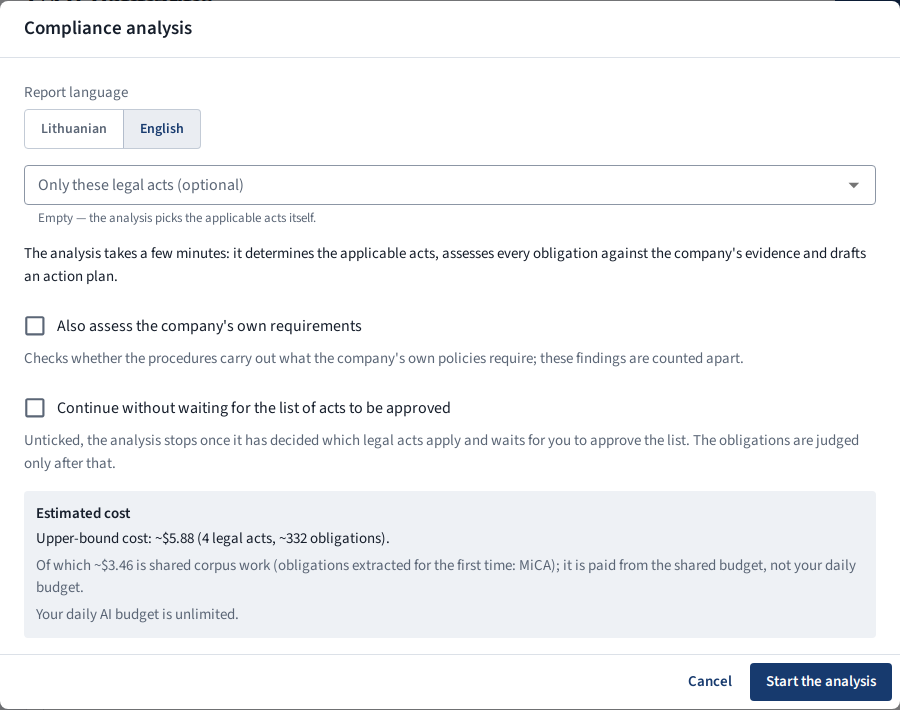
\includegraphics[width=.58\textwidth]{figures/screens/analysis-start-dialog}
\caption{Pradžios dialogas. Po parinktimis pateikiamas kainos įvertis iš
\route{GET}{/api/reports/estimate}: viršutinė kainos riba su aktų ir pareigų skaičiumi, dalis,
kuri yra vienkartinis teisės aktų bazės darbas, apmokamas iš bendro biudžeto, ir naudotojo
dienos biudžetas.}\label{fig:console:start}
\end{figure}

Prieš žmogui patvirtinant, dialogas paprašo API kainos įverčio ir parodo \emph{viršutinę} vykdymo
kainos ribą, kiek aktų ir pareigų jis apima, kiek iš jos tenka vienkartiniam darbui su teisės
aktų baze (pirmą kartą išskiriamoms pareigoms), kuris apmokamas iš bendro, o ne naudotojo
biudžeto, ir likusį naudotojo dienos biudžetą. Kai modelio kaina nežinoma, skaičius yra apatinė
riba ir užrašomas su žodžiais \enquote{mažiausiai}. Likusį biudžetą viršijantis įvertis sukelia
įspėjimą, bet neblokuoja: API atsisako pradėti tik tada, kai dienos biudžetas beveik išnaudotas,
o pradėtas vykdymas niekada nestabdomas pusiaukelėje. Tris API atsisakymus dialogas rodo savo viduje,
išverstus: tuščia teisės aktų bazė, šios įmonės analizė jau vykdoma ar laukia (su nuoroda į ją)
ir išnaudotas biudžetas. Kaip skaičiuojamas įvertis, aprašyta \cref{ch:report}; biudžetas ---
\cref{ch:models}.

\paragraph{Apimties ekranas.} Su peržiūra pradėta ataskaita sustoja būsenoje \ui{Laukia apimties
patvirtinimo}. Tada jos puslapis atsiveria skiltyje \ui{Teisės aktai}, kuri tampa patvirtinimo
ekranu (\file{pages/Reports/ReportScope.jsx}, \cref{fig:console:scope}). Aktai pateikti grupėse,
į kurias juos sudėjo vykdymas, kiekviena kortelė su modelio verdiktu, pasitikėjimu, motyvais ir
cituotomis taikymo srities nuostatomis, ir jungikliu \ui{Vertinti}, kurio pradinė padėtis
atitinka vykdymo sprendimą. Įjungus aktą, kuris įmonės nesaisto, jis vertinamas kaip geroji
praktika; išjungus taikomą aktą, jis paliekamas nuošalyje; kortelė tai pasako žodžiais. Po
kiekvieno jungiklio perjungimo, po trumpos pauzės, API klausiama antrosios dalies kainos tokiam
pasirinkimui (tas pats \route{POST}{/api/reports/{id}/scope} be \code{approved}, kuris nieko
neišsaugo). \ui{Patvirtinti ir tęsti} išsiunčia sprendimą su \code{approved: true}, ir vykdymas
tęsiamas; \ui{Atšaukti analizę} jį baigia. Jungiklių padėtis laikoma naršyklės skirtuke, kol
žmogus žiūri kitur. Ataskaita ir jos eksportas vėliau nurodo, kas ir kada patvirtino sąrašą, ir
atskirai išskiria aktus, dėl kurių nuspręsta priešingai verdiktui.

\begin{figure}[htbp]
\centering
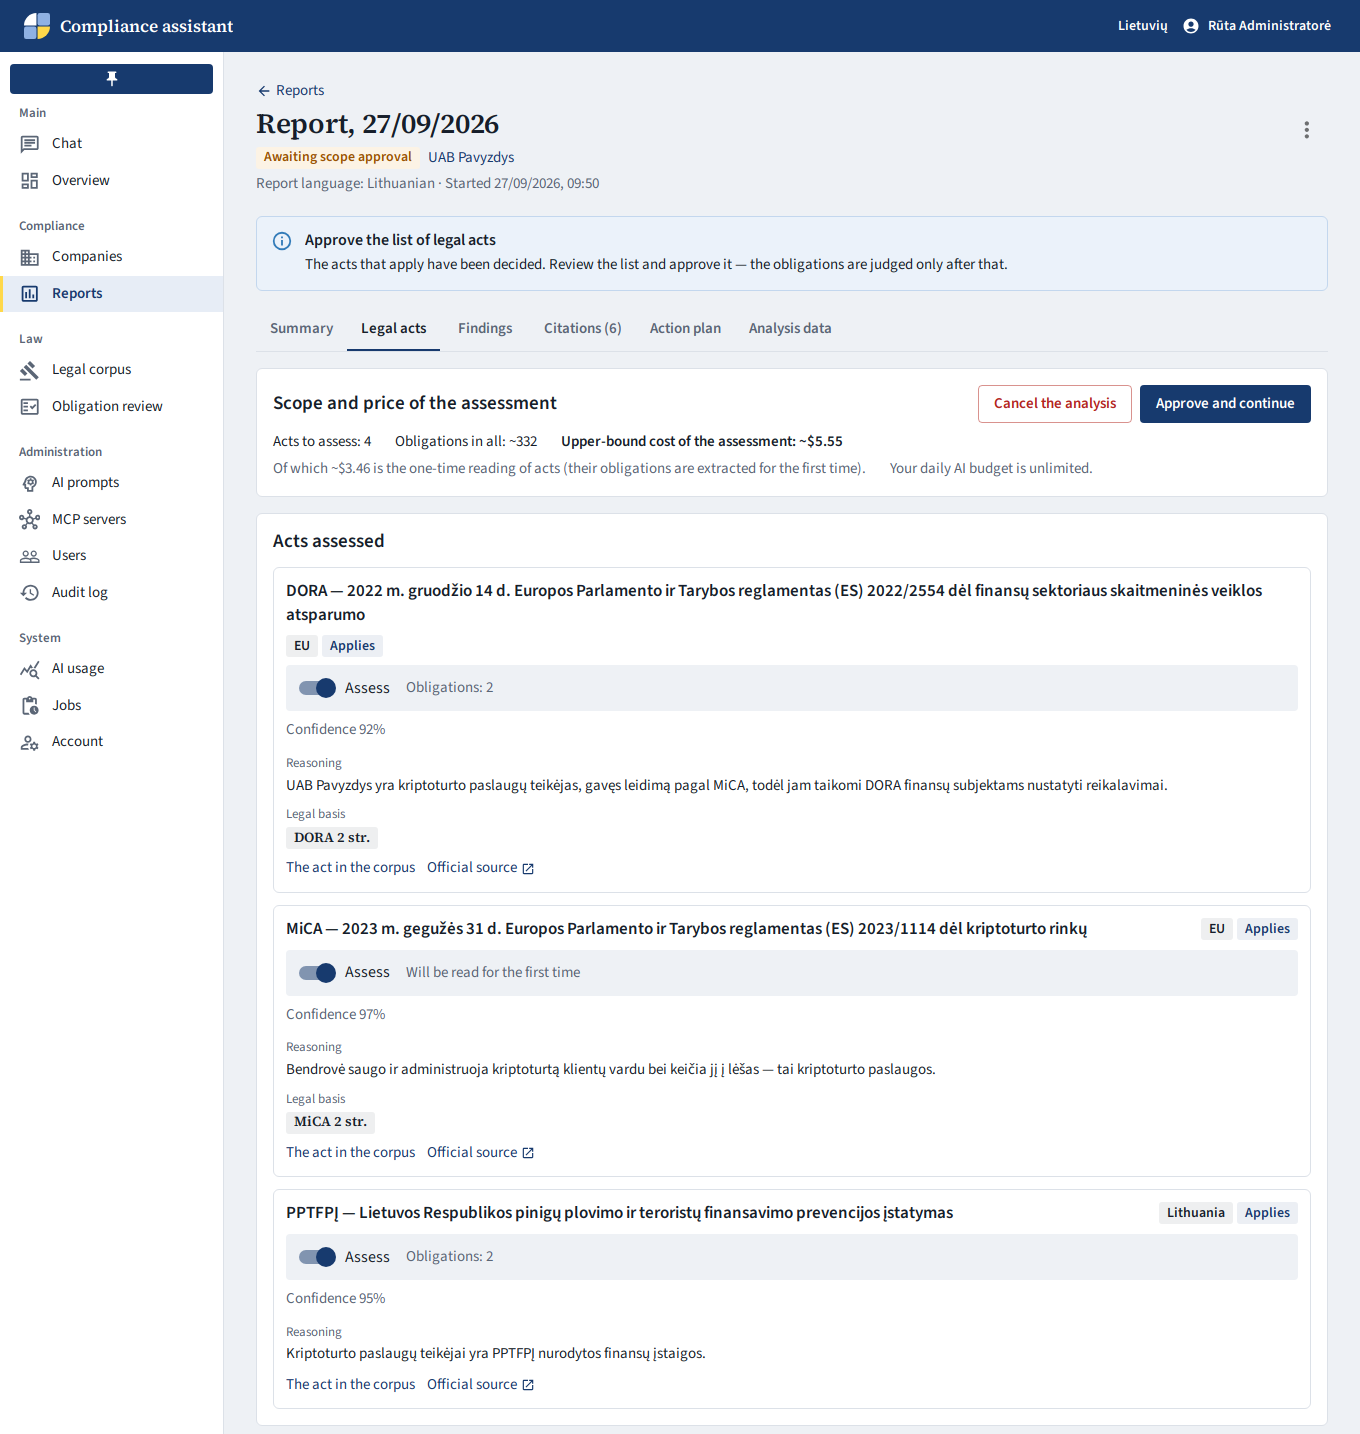
\includegraphics[width=.76\textwidth, trim=240 539 0 52, clip]{figures/screens/report-scope}
\caption{Ataskaita, laukianti apimties patvirtinimo. Juosta pasako, ko prašoma; kainos skydelyje
yra du mygtukai; kiekvienas aktas turi savo jungiklį \ui{Vertinti} su pareigų skaičiumi, kurį jis
atneštų, arba užrašu \enquote{Bus perskaitytas pirmą kartą}, kai jo pareigos dar
neišskirtos.}\label{fig:console:scope}
\end{figure}

\paragraph{Kol ji vykdoma.} Eilėje laukianti ar vykdoma ataskaita rodo eigos kortelę
(\file{pages/Reports/ReportProgress.jsx}): šio vykdymo etapus su jų būsena ir trukme, kiekvieną
baigtą etapą su jo modeliu ir kaina, iki šiol patirtas DI sąnaudas ir praėjusį laiką.
\ui{Stabdyti analizę} ją sustabdo kitame etape; jau išleisti pinigai negrąžinami. Etapai
priklauso užduočiai, o paprastas naudotojas mato tik savo pradėtas užduotis, todėl
administratoriaus pradėta ataskaita rodo eigos eilutę be etapų ir paaiškina kodėl.

\paragraph{Baigta ataskaita.} Baigta ataskaita turi šešias skiltis (\code{TABS} faile
\file{ReportDetail.jsx}): \ui{Santrauka}, \ui{Teisės aktai}, \ui{Išvados}, \ui{Nuorodos},
\ui{Veiksmų planas} ir \ui{Analizės duomenys} (įmonės profilis, koks jis buvo užfiksuotas
vykdymui, --- po apimties peržiūros toks, kokį jį perskaitė antroji vykdymo dalis).
Virš jų yra patvirtinimas ir, kai ataskaitos naudotas aktas nuo to laiko turi
naujesnę redakciją, įspėjimas \ui{Teisės aktai atnaujinti} su mygtuku \ui{Paleisti iš naujo}.

\begin{figure}[htbp]
\centering
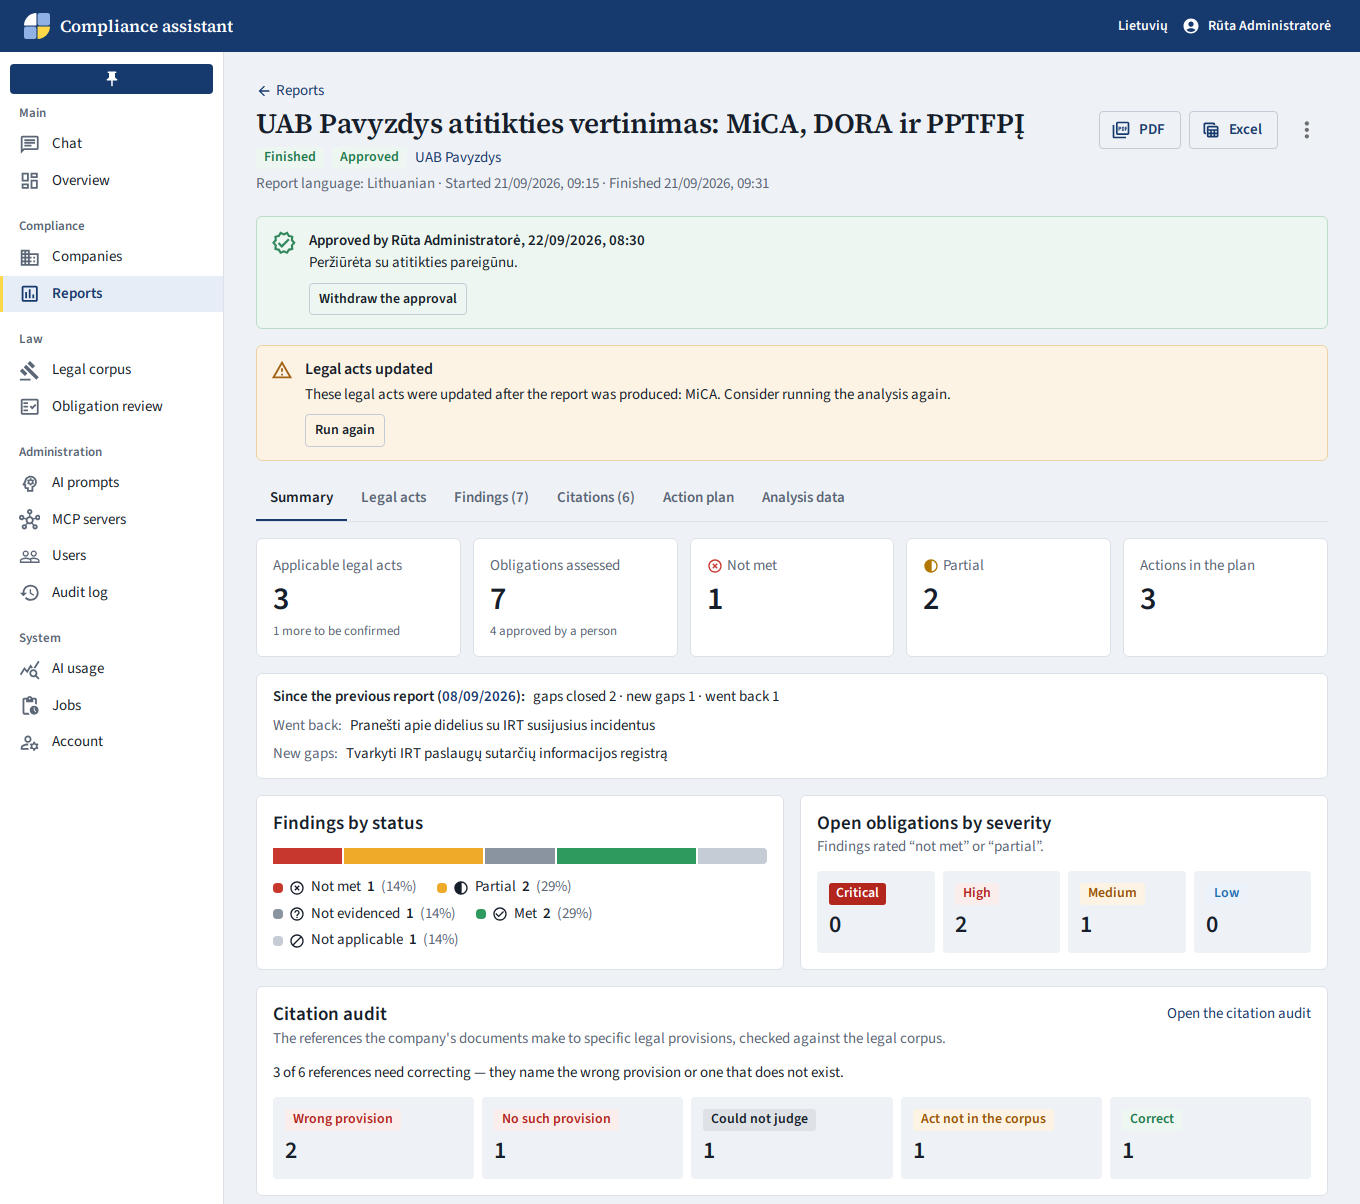
\includegraphics[width=.72\textwidth, trim=240 234 0 52, clip]{figures/screens/report-overview}
\caption{Baigtos, patvirtintos ataskaitos santraukos skiltis. Iš viršaus: patvirtinimo juosta su
\ui{Atšaukti patvirtinimą}; įspėjimas, kad aktas po vykdymo atnaujintas; plytelės; kas
pasikeitė nuo ankstesnės ataskaitos; išvados pagal būseną viena juosta; neįvykdytos pareigos
pagal reikšmingumą. Žemiau eina teisės aktų nuorodų patikros
skaičiai.}\label{fig:console:overview-report}
\end{figure}

Santrauka (\file{ReportOverview.jsx}, \cref{fig:console:overview-report}) yra tai, ką valdybos
narys perskaito pirmiausia: įvertinti aktai ir pareigos ir kiek iš tų pareigų buvo patvirtinęs
žmogus, penkių būsenų skaičiai, neįvykdytos pareigos pagal reikšmingumą, kas pasikeitė nuo
įmonės ankstesnės ataskaitos, aktai, nevertinti, nes jų taikytinumą dar reikia patvirtinti (su
keliu į jų klausimus), pasirengimas aktams, kurie bus taikomi vėliau, teisės aktų nuorodų
patikros skaičiai, modelio parengta santrauka ir kilmė --- instrukcijų versijos, modeliai ir aktų
redakcijos, iš kurių gimė ataskaita, bei jos DI sąnaudos. Skaičiai yra šios dienos rezultatas:
jie apima įmonei galiojančius aktus, atsižvelgia į peržiūrėtojo sprendimą, kur jis yra, ir
neapima įmonės vidaus reikalavimų, kurie skaičiuojami atskirai.

Teisės aktų skiltis (\file{ReportActs.jsx}) rodo, ką ataskaita padarė su kiekvienu aktu, ---
įvertino, įvertino kaip pasirengimą vėlesnei datai, nevertino, kol nebus atsakyta į klausimą,
--- o suskleistuose sąrašuose --- direktyvas, aktus, kurie tik organizuoja institucijos veiklą,
aktus, kurie pripažinti netaikomais, ir tuos, kuriuos atrankoje atmetė katalogas. Po vykdymo
atnaujintas aktas pažymimas savo kortelėje.

\paragraph{Išvados ir peržiūros dialogas.} Išvadų skiltis (\file{ReportFindings.jsx}) grupuoja
išvadas pagal aktą arba sritį, filtruoja jas pagal būseną ir reikšmingumą ir ieško jų tekste.
Kortelė rodo būsenos ir reikšmingumo žymes, \ui{Peržiūrėta}, kai žmogus pakeitė modelio
vertinimą, ir \ui{Nepatvirtinta pareiga}, kai pačios pareigos žmogus niekada nepatvirtino
(\cref{fig:console:finding}). Atverta ji pateikia pareigą akto žodžiais (šriftu su užraitomis,
kaip ir visa, kas cituojama iš šaltinio), vertinimą, priežastį, kai ją užrašė peržiūrėtojas,
pasekmę --- akte numatytas maksimalias sankcijas, visada su pastaba, kad tai riba, o ne prognozė,
--- įrodymus su citatomis, rekomendaciją ir terminą, peržiūrėtojo pastabą ir ankstesnius tos
pačios pareigos vertinimus įmonės ankstesnėse ataskaitose. Geltonu žymekliu pažymėta citata
atveria dokumento stalčių jos vietoje.

\begin{figure}[htbp]
\centering
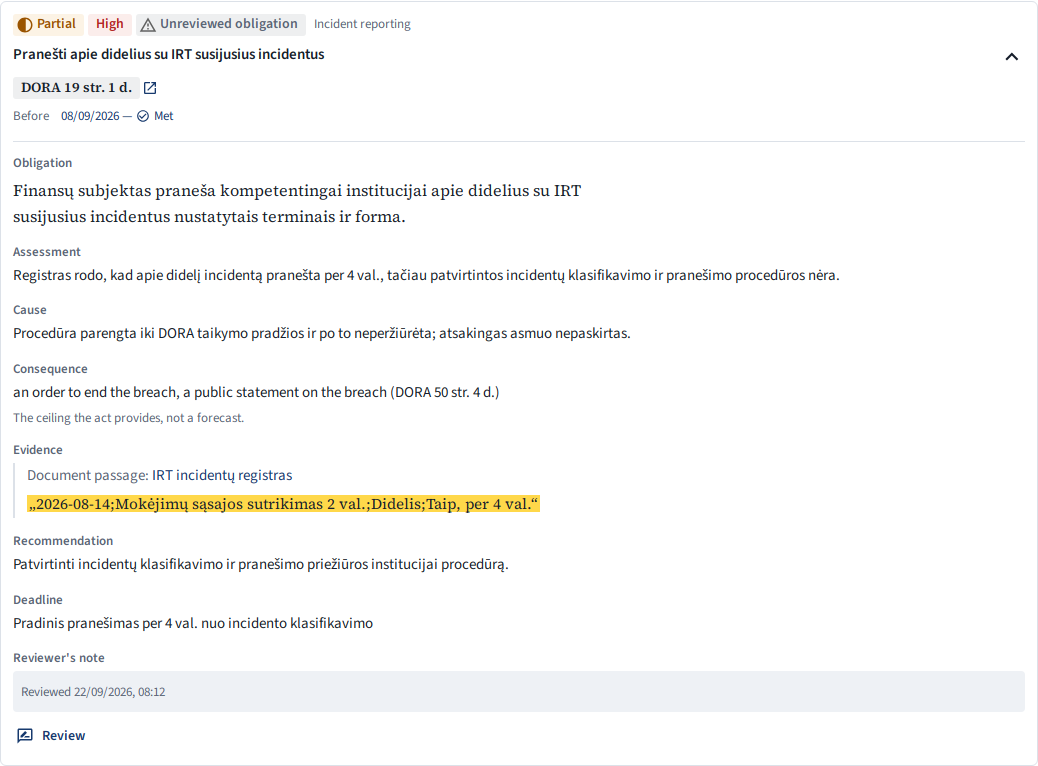
\includegraphics[width=.505\textwidth]{figures/screens/report-finding-card}\hfill
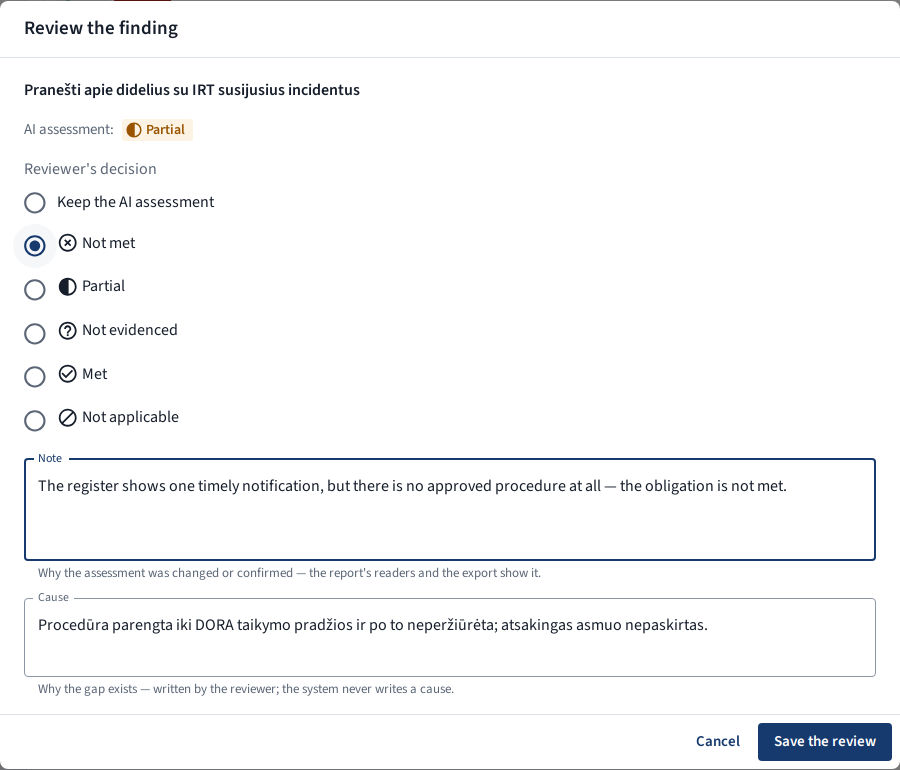
\includegraphics[width=.475\textwidth]{figures/screens/finding-review-dialog}
\caption{Kairėje --- viena atverta išvada: žymės, ankstesnis vertinimas (\ui{Anksčiau}), pareiga,
vertinimas, priežastis, pasekmė su pastaba \enquote{riba, o ne prognozė}, geltonu žymekliu
pažymėta įrodymo ištrauka ir \ui{Peržiūrėti}. Dešinėje --- peržiūros dialogas: DI vertinimas
lieka matomas; peržiūrėtojas jį palieka arba pasirenka kitą būseną, parašo pastabą ir
priežastį, kurios sistema niekada nerašo.}\label{fig:console:finding}
\end{figure}

\ui{Peržiūrėti} atveria peržiūros dialogą (\file{FindingReviewDialog.jsx}). Modelio verdiktas
lieka matomas; peržiūrėtojas jį arba palieka (\ui{Palikti DI vertinimą}), arba pasirenka kitą iš
penkių būsenų ir parašo pastabą. Dialoge taip pat yra laukas \ui{Priežastis}: kodėl atsirado
spraga. Priežastis yra vienintelė išvados dalis, kurią rašo tik žmogus, --- dokumentai rodo, ko
trūksta, bet ne kodėl, --- todėl jos nepildo nei analizė, nei pokalbių asistentas. Dialogas
siunčia \route{PATCH}{/api/reports/{id}/findings/{fid}}; būsena, kurią paskui rodo kiekvienas
vaizdas ir eksportas, yra peržiūrėtojo sprendimas, o bet kokia peržiūra serveryje atšaukia
ataskaitos patvirtinimą.

\paragraph{Teisės aktų nuorodų patikra.} Skiltis \ui{Nuorodos} (\file{ReportCitations.jsx},
\cref{fig:console:citations}) išvardija kiekvieną įmonės dokumentų nuorodą į konkrečią nuostatą,
patikrintą vykdant ataskaitą (\cref{ch:company,ch:report}). Kiekviena kortelė turi verdiktą ---
\ui{Teisinga}, \ui{Ne ta nuostata}, \ui{Tokios nuostatos nėra}, \ui{Akto nėra bazėje} arba
\ui{Nepavyko įvertinti}, --- dokumentą, nuorodą taip, kaip ji parašyta, su tuo, ką, dokumento
teigimu, ji apima, o esamos nuostatos atveju --- jos tikrąją antraštę, patikros pastabą, ištrauką
ir nuorodas. Pirmiausia rodomos problemos; perjungikliai su skaičiais filtruoja pagal verdiktą.

\begin{figure}[htbp]
\centering
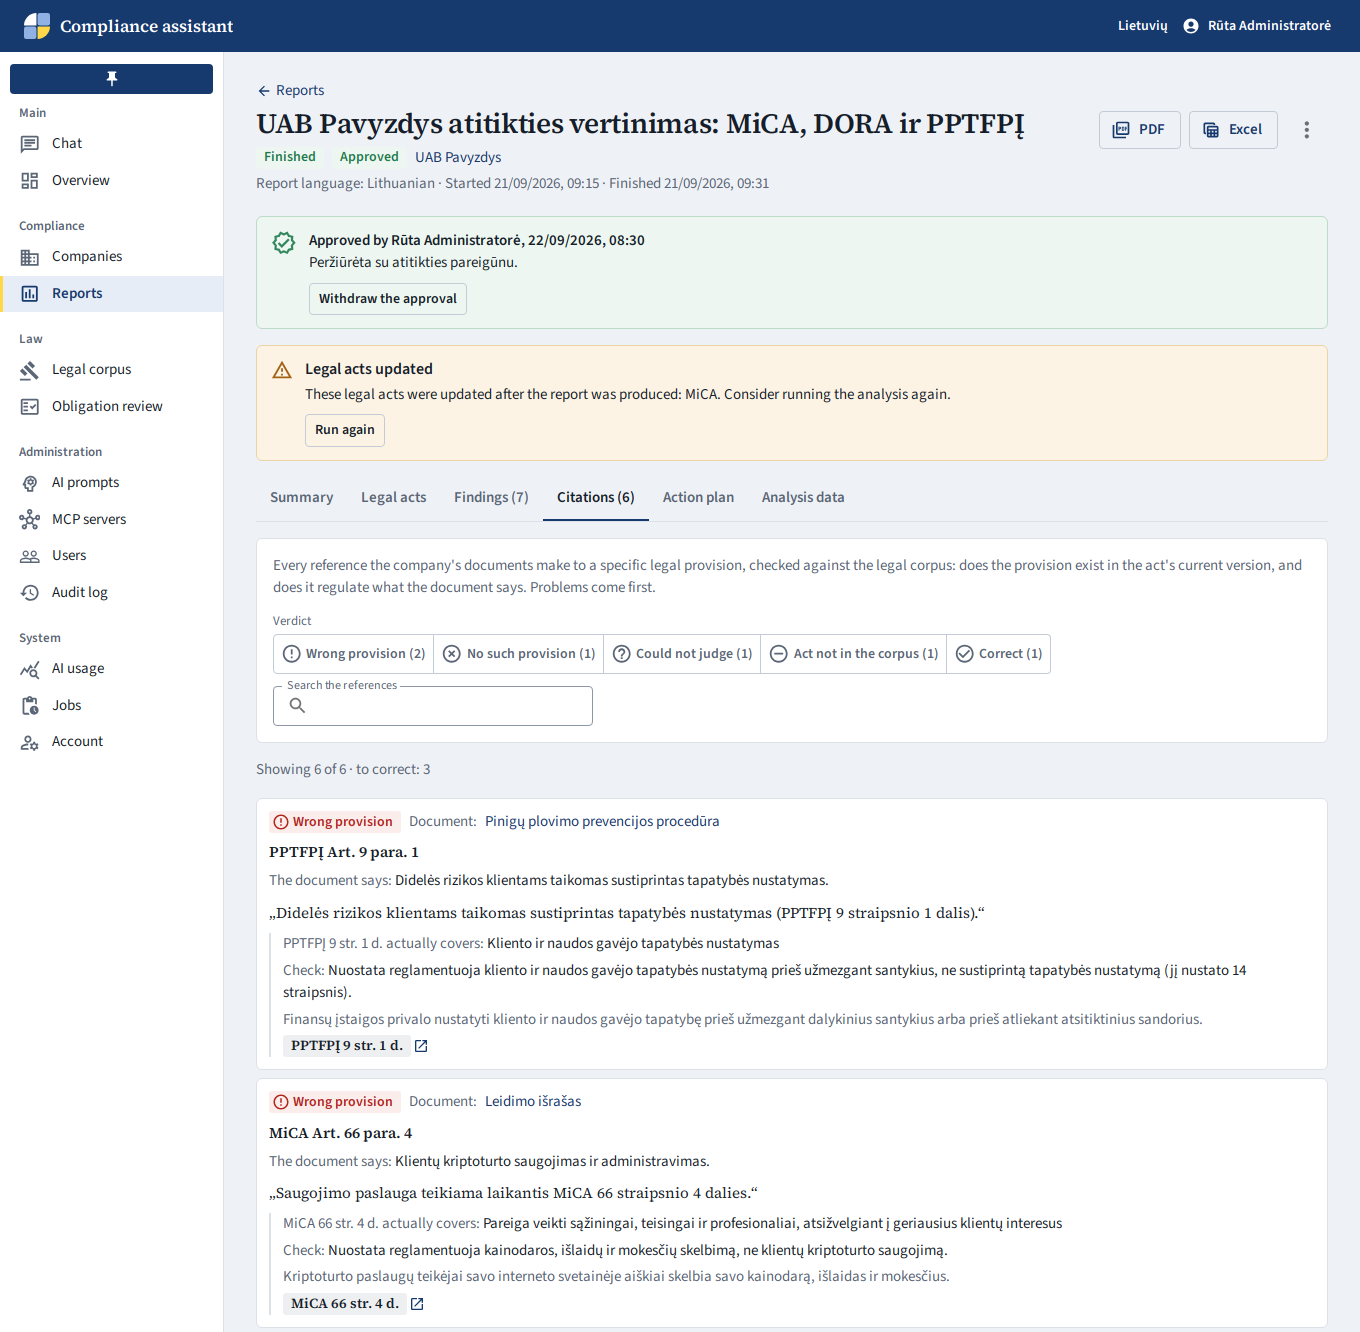
\includegraphics[width=.76\textwidth, trim=240 262 0 52, clip]{figures/screens/report-citations}
\caption{Ataskaitos teisės aktų nuorodų patikra. Kiekviena kortelė pastato tai, ką sako
dokumentas, šalia to, ką cituojama nuostata iš tikrųjų apima, su patikros pastaba ir nuoroda į
nuostatą.}\label{fig:console:citations}
\end{figure}

\paragraph{Veiksmų planas.} Plano skiltis (\file{ReportActionPlan.jsx}) išvardija veiksmus pagal
prioritetą, kiekvieną su aprašymu, laikotarpiu, pastangomis, atsakingu asmeniu ir sritimi;
\ui{Susijusios išvados} atveria išvadų skiltį, susiaurintą iki išvadų, kurias tas veiksmas
uždaro. Veiksmas, kuris tik rengia dar negaliojančiam aktui, pažymimas kaip pasirengimas ir
pateikiamas paskutinis.

\paragraph{Patvirtinimas ir eksportas.} \ui{Patvirtinti ataskaitą} baigtos ataskaitos antraštėje
atveria dialogą, kuris paaiškina, ką reiškia patvirtinimas, --- žmogus peržiūrėjo išvadas ir
planą, o bet koks vėlesnis išvados pakeitimas patvirtinimą atšaukia, --- ir priima neprivalomą
pastabą (\file{ReportApproval.jsx}, \route{PATCH}{/api/reports/{id}} su \code{approved: true}).
Jis taip pat pasako, kad patvirtinimas pajudina įmonės veiksmų registrą; po to pasirodantis
pranešimas žodžiais nusako, kas pasikeitė (pridėti veiksmai, praleisti veiksmai, nes juos jau
apima kitas, pareigos, kurių įvykdymas patvirtintas, uždaryti arba vėl į darbą grąžinti ankstesni
veiksmai), su nuoroda į registrą. Patvirtinta ataskaita rodo žalią juostą su tuo, kas ją
patvirtino, kada, pastaba ir mygtuku \ui{Atšaukti patvirtinimą}. Antraštėje taip pat yra
eksportas, \ui{PDF} ir \ui{Excel}, atsisiunčiamas su sesijos prieigos raktu
(\route{GET}{/api/reports/{id}/export?format=pdf|xlsx}); kas yra failuose, aprašyta
\cref{ch:report}.

\subsection{Veiksmų registras ir teisės aktų pokyčiai}\label{sec:console:register}

\begin{figure}[htbp]
\centering
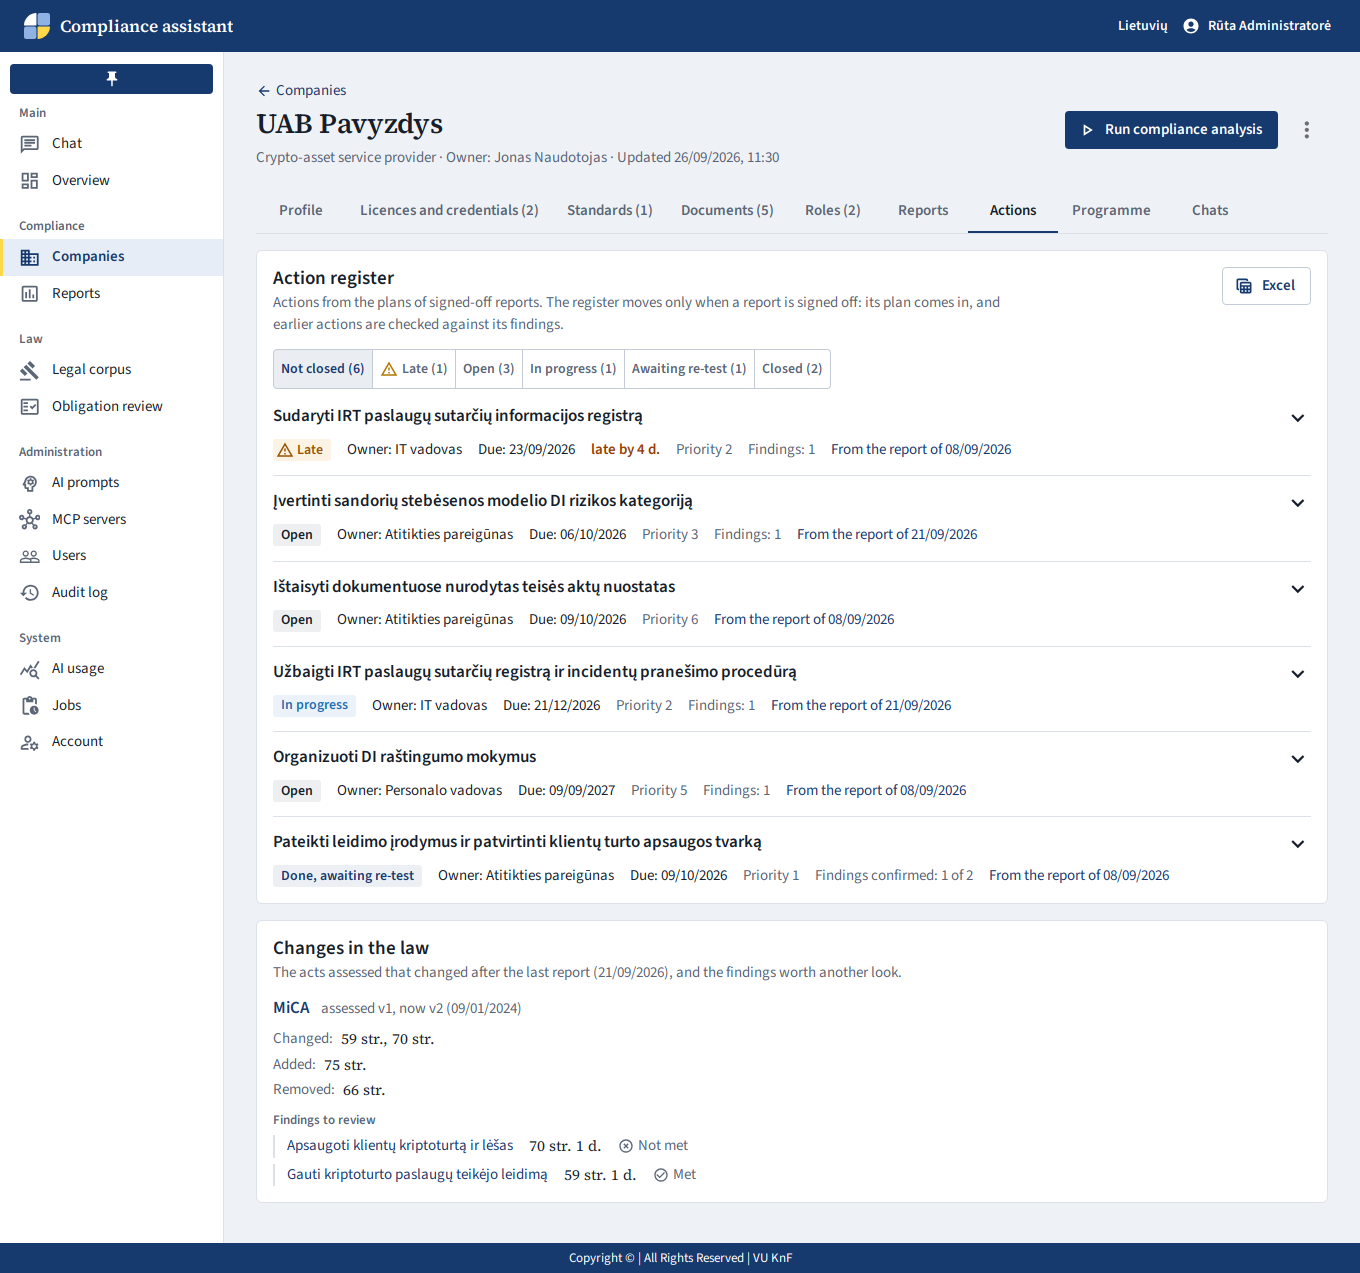
\includegraphics[width=.66\textwidth, trim=240 30 0 52, clip]{figures/screens/action-register}
\caption{Įmonės skiltis \ui{Veiksmai}. Perjungikliai skaičiuoja ir filtruoja veiksmus pagal
būseną (vėluojantis --- su įspėjimo ženklu, niekada ne vien spalva); kiekviena eilutė pateikia
atsakingą asmenį, terminą, prioritetą, išvadas ir ataskaitą, iš kurios veiksmas kilo. Po
registru --- \ui{Teisės aktų pokyčiai}: aktas, pasikeitęs nuo paskutinės ataskaitos, jo
pakeistos, pridėtos ir pašalintos nuostatos ir jomis besiremiančios
išvados.}\label{fig:console:register}
\end{figure}

Įmonės skiltis \ui{Veiksmai} (\file{CompanyActions.jsx}, \cref{fig:console:register}) yra
\term{veiksmų registras}: tai, ko reikalavo patvirtintų įmonės ataskaitų planai, išsaugota ir po
ataskaitų. Kortelė po savo pavadinimu pasako, kad registras juda tik tada, kai patvirtinama
ataskaita, nes šioje skiltyje niekas veiksmo neprideda. Perjungikliai skaičiuoja ir filtruoja
veiksmus pagal būseną: \ui{Neuždaryti}, \ui{Vėluoja}, \ui{Atviri}, \ui{Vykdomi}, \ui{Laukia
patikros} ir \ui{Uždaryti}. \enquote{Vėluoja} nėra būsena, kurią nustato žmogus; ji rodoma
atviram ar vykdomam veiksmui, kurio terminas praėjo.

Atverta eilutė (\file{ActionRow.jsx}) išvardija išvadas, kurias veiksmas turi uždaryti,
kiekvieną pažymėdama \enquote{patvirtinta}, kai vėlesnė patvirtinta ataskaita jos pareigą rado
įvykdytą, ir turi formą, kuria žmogus veiksmą prižiūri: atsakingas asmuo, terminas, būsena
(atviras, vykdomas, įvykdytas, uždarytas) ir pastaba, išsaugoma per \route{PATCH}{/api/actions/{id}}.
\enquote{Įvykdytas, laukia patikros} yra atsakingo asmens žodis ir laukia, kol jį patvirtins vėlesnė ataskaita;
uždarant rankiniu būdu reikia pastabos; ataskaitos uždaryto veiksmo čia negalima atverti iš
naujo --- uždarymas ginčijamas išvadoje, toje ataskaitoje. \ui{Excel} atsisiunčia registrą.

Po registru \ui{Teisės aktų pokyčiai} (\file{LawChanges.jsx}) rodo kiekvieną įmonės naujausios baigtos
ataskaitos įvertintą aktą, kuris dabar turi naujesnę redakciją: perskaitytą ir galiojančią
redakcijas, pakeistas, pridėtas ar pašalintas nuostatas ir ataskaitos išvadas, kurios remiasi
pakeista ar pašalinta nuostata. Taisyklės, pagal kurias juda registras, aprašytos
\cref{ch:register}.

\subsection{Atitikties programa ir jos dokumentai}\label{sec:console:programme}

\begin{figure}[htbp]
\centering
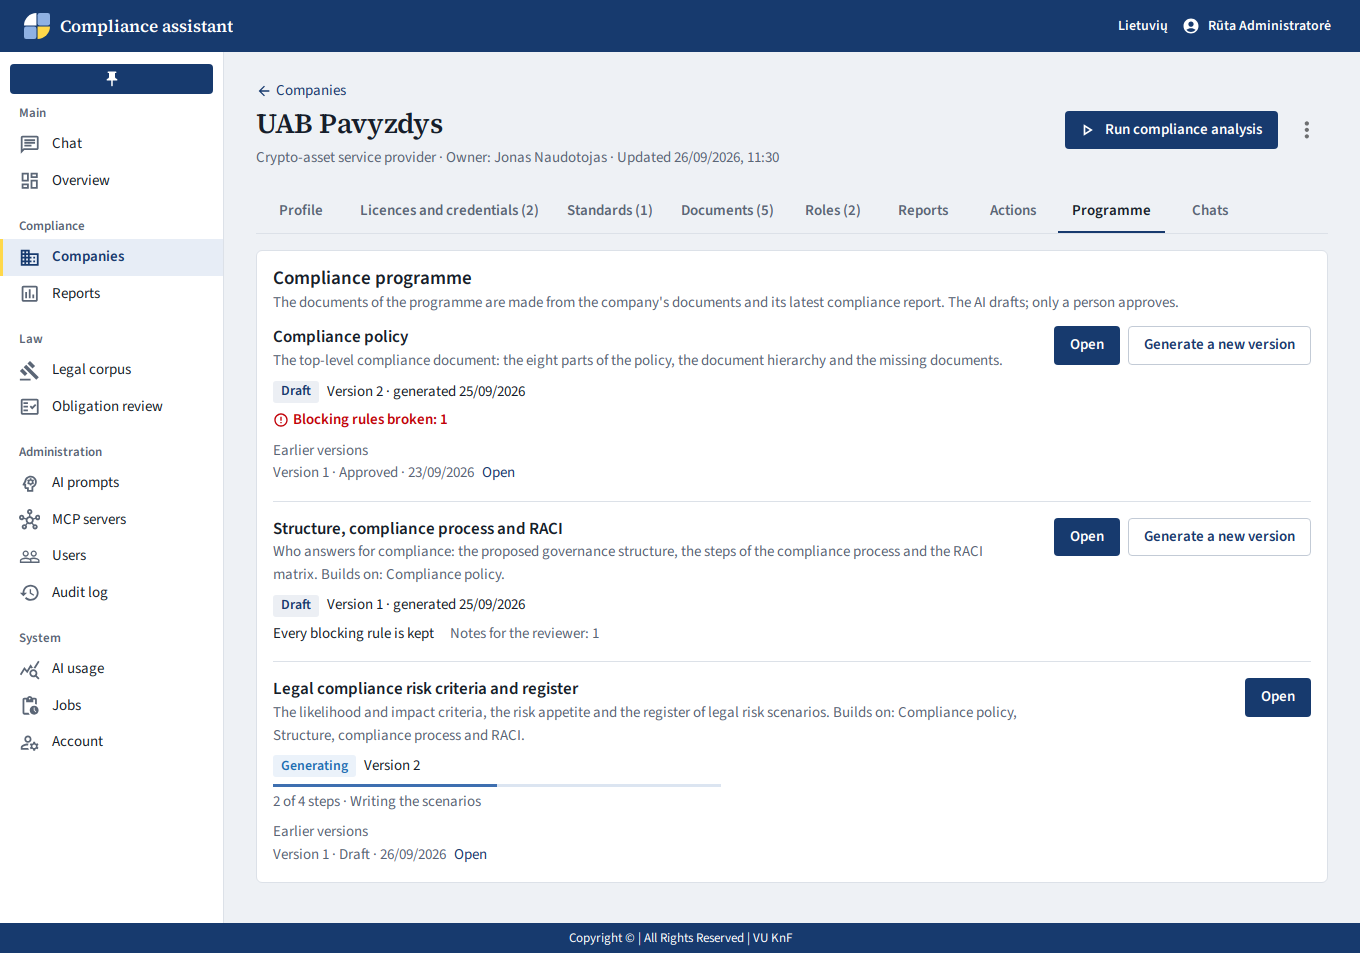
\includegraphics[width=.76\textwidth, trim=240 33 0 52, clip]{figures/screens/programme-tab}
\caption{Įmonės skiltis \ui{Programa}: trys programos dokumentų rūšys ta tvarka, kuria jos
remiasi viena kita, kur yra naujausia kiekvienos versija (projektas, pažeidžiantis vieną
blokuojančią taisyklę, projektas, laikantis jų visų, generuojama versija su savo etapu),
ankstesnės versijos ir būseną atitinkantys mygtukai.}\label{fig:console:programme}
\end{figure}

Skiltis \ui{Programa} (\file{CompanyProgramme.jsx}, \cref{fig:console:programme}) išvardija tris
\term{programos dokumentų} rūšis, kurių projektus sistema rengia įmonei, ta tvarka, kuria kiekviena
remiasi ankstesnėmis: \ui{Atitikties politika}; \ui{Valdymo struktūra, atitikties procesas ir
RACI}; ir \ui{Teisinės atitikties rizikos vertinimo kriterijai ir registras}. Kiekvienai rūšiai
ji rodo, kur yra naujausia versija, --- dar nesugeneruota, laukia eilėje ar generuojama su savo
etapu, projektas su pažeidžiamų blokuojančių taisyklių skaičiumi, patvirtinta (kas ir kada),
nepavykusi ar atšaukta, --- o po ja --- ankstesnes versijas. \ui{Generuoti} arba
\ui{Generuoti naują versiją} pirmiausia paklausia: dialogas pasako, kad generavimas vyksta fone
apie penkias minutes ir išleidžia apie 0,50~\$ dienos DI biudžeto (\code{RUN_COST_USD},
suapvalinta API skaičiaus kopija konsolėje), įvardija rūšis, kuriomis jis remiasi ir kurių dar
nėra, ir prašo dokumento kalbos.

\begin{figure}[htbp]
\centering
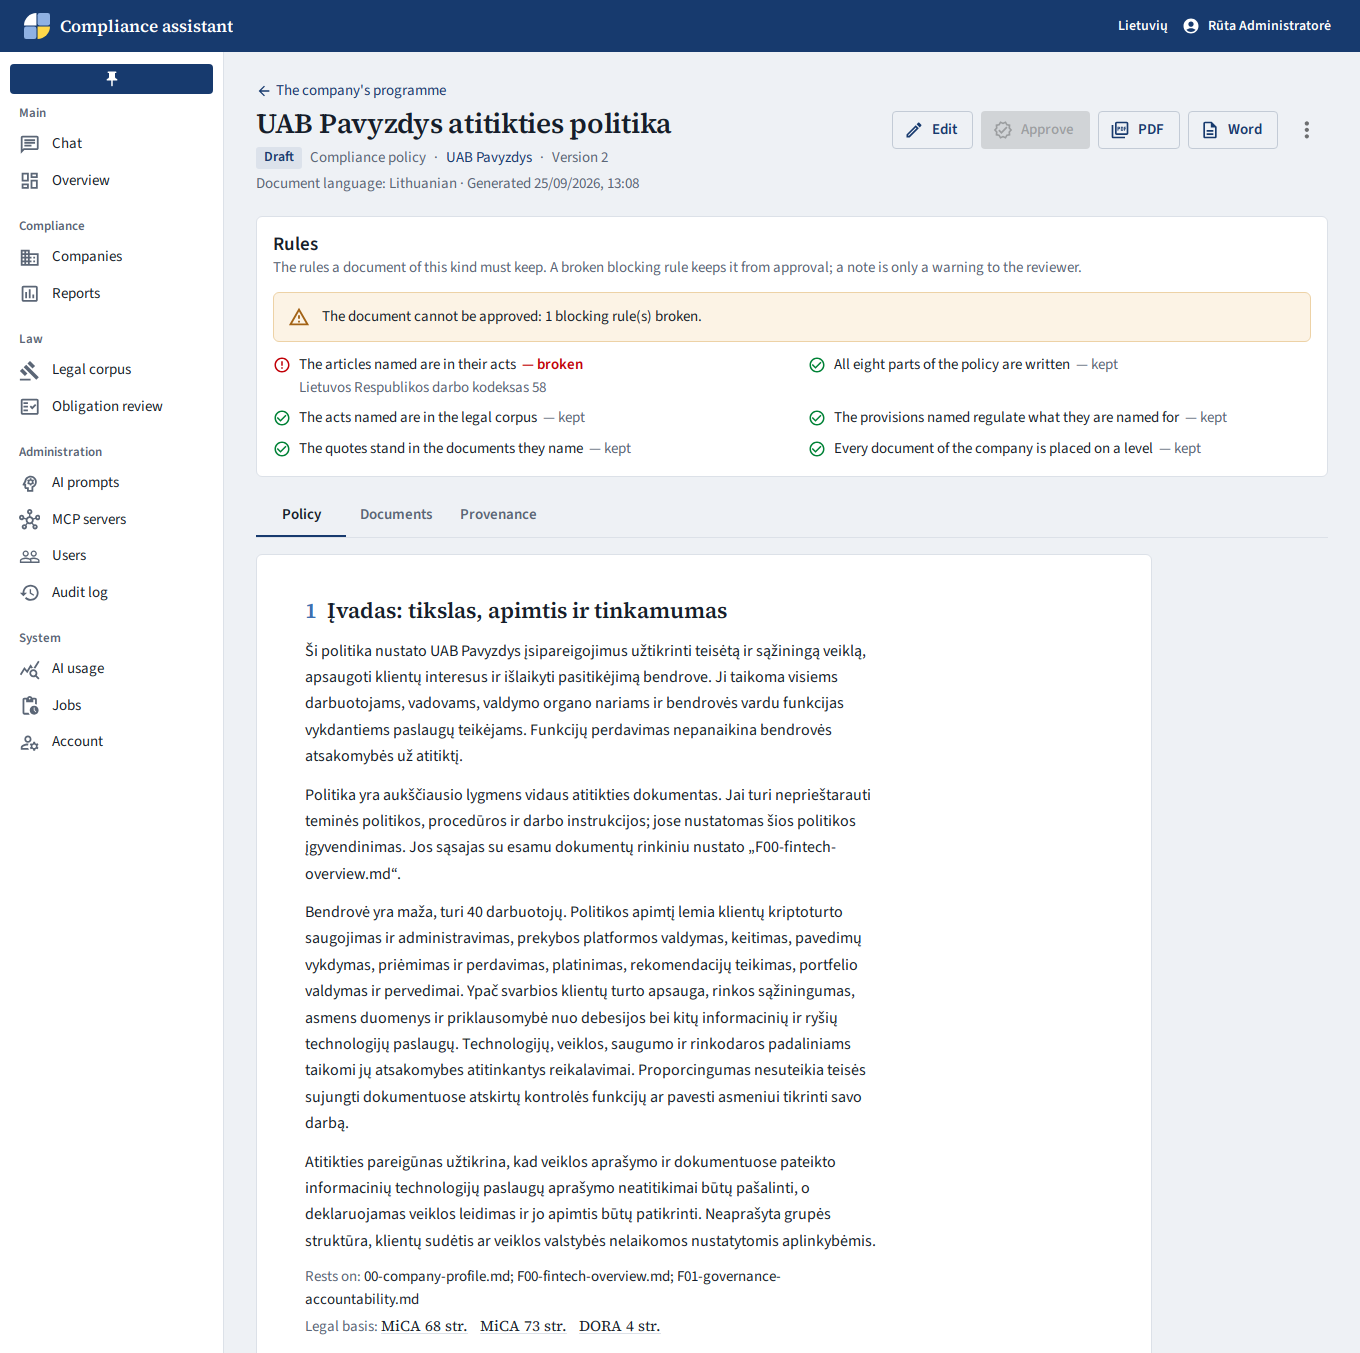
\includegraphics[width=.76\textwidth, trim=240 453 0 52, clip]{figures/screens/product-policy}
\caption{Atitikties politikos projektas (\code{/console/programme/:productId}). \ui{Patvirtinti}
išjungtas, nes skydelis \ui{Taisyklės} rodo vieną pažeistą blokuojančią taisyklę (nurodytas
straipsnis, kurio akte nėra). Žemiau --- politikos skiltys ir jos pirmosios dalies
pradžia.}\label{fig:console:product}
\end{figure}

\ui{Atidaryti} veda į vieno programos dokumento puslapį (\file{pages/Programme/ProductPage.jsx},
\cref{fig:console:product}). Jo antraštė nurodo būseną --- \ui{Generuojama}, \ui{Projektas},
\ui{Patvirtinta}, --- rūšį, įmonę ir versiją, ir joje yra veiksmų mygtukai. Po ja yra skydelis
\ui{Taisyklės} (\file{RulesPanel.jsx}): serverio pusė kiekvieną dokumentą tikrina pagal jo rūšies
taisykles, o skydelis išvardija kiekvieną taisyklę kaip laikomą ar pažeistą; pažeista taisyklė yra arba
blokuojanti (ji neleidžia dokumento patvirtinti), arba pastaba peržiūrėtojui, su
paaiškinimu, kas ją pažeidė. Žemiau --- turinys skiltyse, kurios priklauso nuo rūšies
(\code{KIND_TABS} faile \file{programmeUtils.js}), o kiekviena rūšis baigiasi skiltimi
\ui{Kilmė}: iš ko dokumentas padarytas, kurios instrukcijos ir modeliai jį parašė ir kiek kainavo
vykdymas.

\begin{table}[H]
\caption{Programos dokumento puslapio skiltys pagal rūšį.}\label{tab:console:producttabs}
\begin{tabularx}{\textwidth}{@{}L{30mm}YL{30mm}@{}}
\toprule
\hd{Rūšis} & \hd{Skiltys} & \hd{Eksportas} \\
\midrule
\code{policy} & \ui{Politika}, \ui{Dokumentai}, \ui{Kilmė} &
PDF, Word \\
\code{governance} & \ui{Struktūra}, \ui{Procesas ir RACI},
\ui{Pareigybės ir spragos}, \ui{Kilmė} & PDF \\
\code{risks} & \ui{Registras}, \ui{Kriterijai}, \ui{Kilmė} & PDF, Excel \\
\bottomrule
\end{tabularx}
\end{table}

\begin{figure}[htbp]
\centering
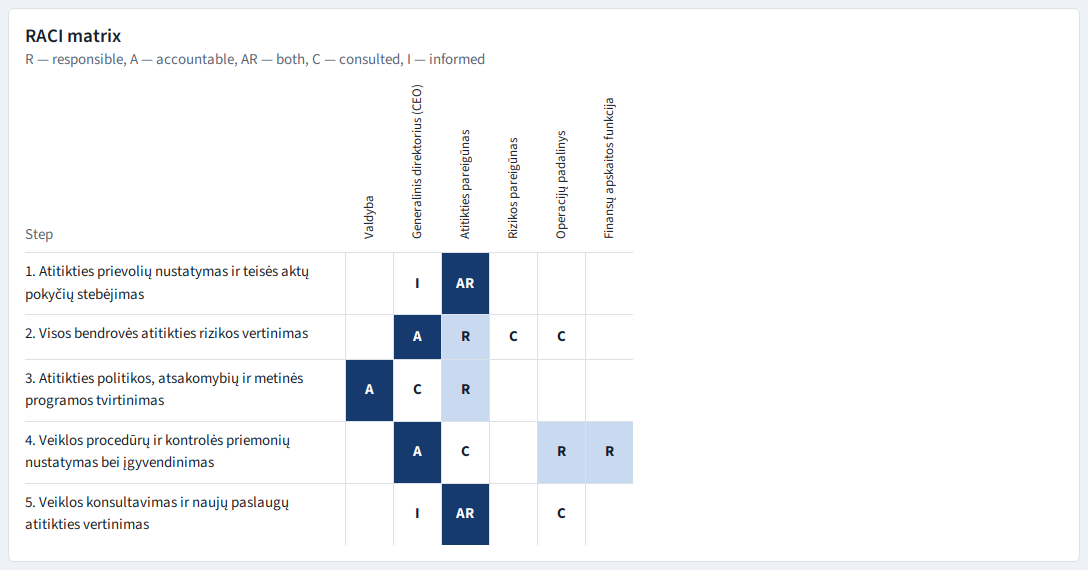
\includegraphics[width=.52\textwidth, trim=0 0 440 0, clip]{figures/screens/governance-raci}

\medskip
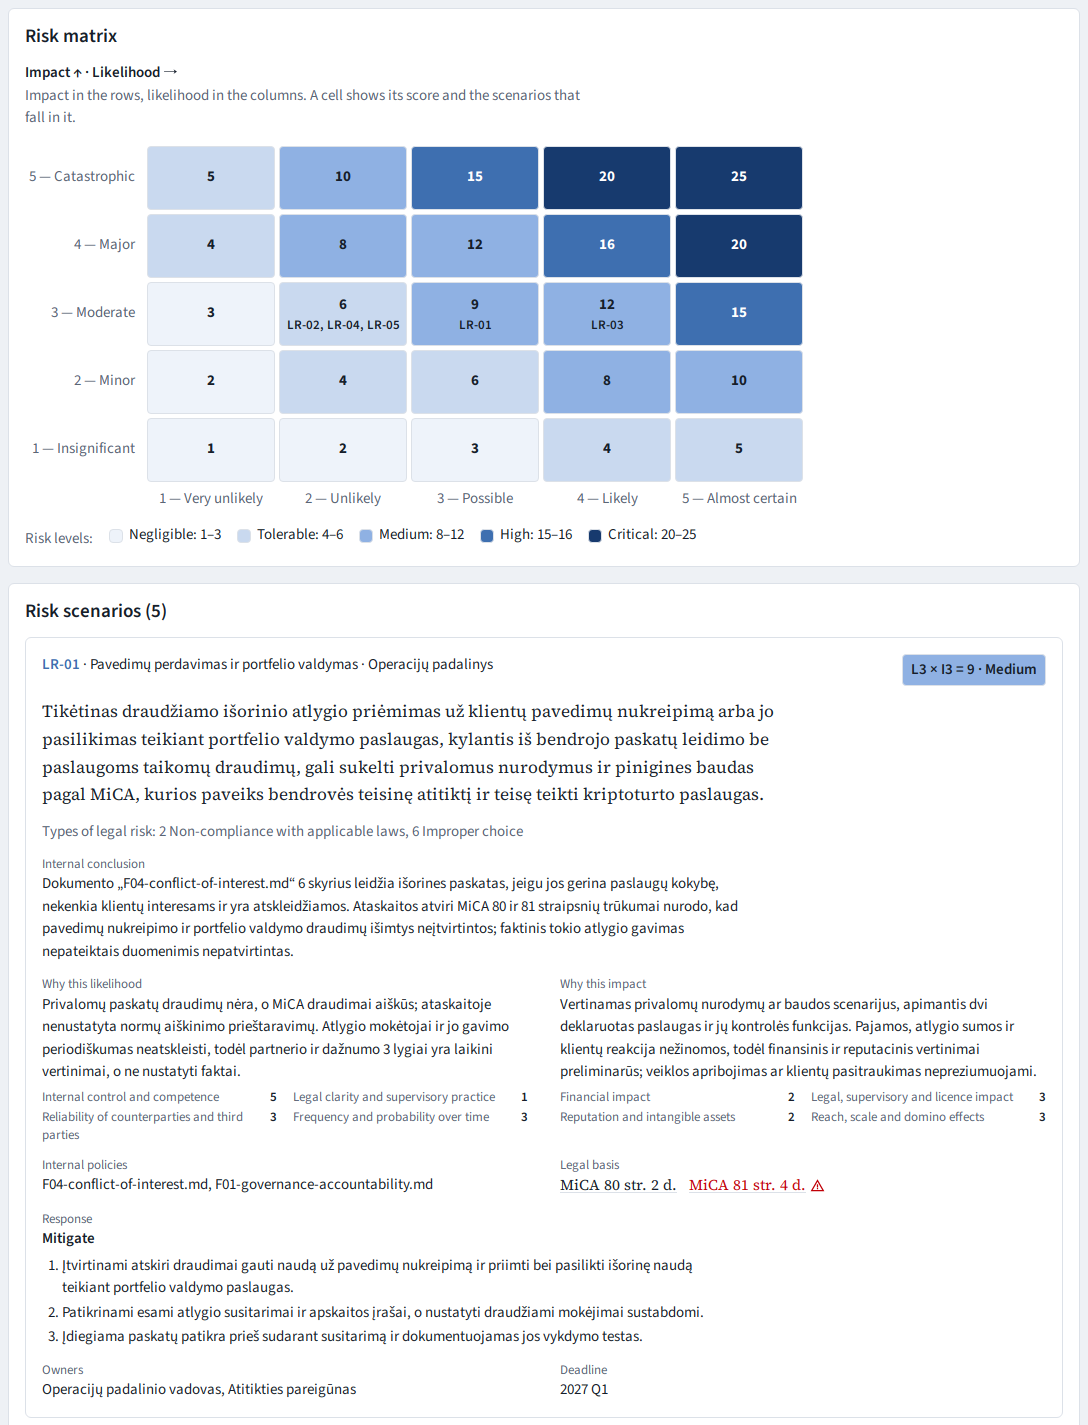
\includegraphics[width=.62\textwidth]{figures/screens/risk-register}
\caption{Dvi programos dokumentų puslapių iškarpos. Viršuje --- valdymo dokumento RACI matrica:
etapai eilutėse, rolės stulpeliuose, kiekvienas etapas su lygiai viena atskaitinga role (A arba
AR) ir bent viena atsakinga (R). Apačioje --- rizikos registras: 5×5 matrica su penkiomis zonomis
ir vienas scenarijus su aštuoniais matmenų balais ir sistemos apskaičiuotu balu
\enquote{T3 × P3 = 9 · Vidutinė}; cituota
nuostata, kurios sistema negalėjo patvirtinti, pažymėta įspėjimo
ženklu.}\label{fig:console:productparts}
\end{figure}

\paragraph{Redagavimas ir patvirtinimas.} \ui{Redaguoti} projekto turinį paverčia formomis:
politikos dalys, dokumentų lygmenys, struktūros mazgai, proceso etapai, RACI langeliai,
scenarijai su balais ir planais, kriterijai. Pakeitimai lieka puslapyje, kol \ui{Išsaugoti
pakeitimus} išsiunčia visą turinį (\route{PUT}{/api/programme/{id}/content}) arba
\ui{Atmesti pakeitimus} juos išmeta. Atsakymas yra turinys tokiu pavidalu, kokiu serveris jį išsaugojo ir
patikrino, ir jis pakeičia tai, kas ekrane, todėl taisyklių skydelis paskui parodo bet kurią
taisyklę, kurią pakeitimas pažeidė ar ištaisė. Puslapis pats niekada neskaičiuoja balo, lygio ar
zonos: pakeistą balą išsaugant perskaičiuoja serveris. \ui{Patvirtinti} yra žmogaus veiksmas
(\file{ProductApproval.jsx}): jis išjungtas, nurodant priežastį, kol pažeista blokuojanti
taisyklė ar yra neišsaugotų pakeitimų, ir jis užfiksuoja dokumentą --- patvirtinto dokumento
patvirtinimo atšaukti negalima, jį galima tik nukopijuoti mygtuku \ui{Nauja versija} į naują
projektą. Eksportas, po vieną mygtuką kiekvienam rūšies formatui (\cref{tab:console:producttabs}),
pateikia projektą ar patvirtintą dokumentą kaip failą, kurio viršelis pasako, kuris tai yra.
Ką daro generavimas ir kokios yra taisyklės, aprašyta \cref{ch:programme}.

\subsection{Teisės aktų bazė}\label{sec:console:corpus}

\ui{Teisės aktų bazė} (\file{pages/Corpus/Corpus.jsx}) atvira kiekvienam naudotojui, nes tai
vieša teisė; administratorius papildomai gauna jos keitimo funkcijas. Ji turi tris skiltis:

\begin{description}
  \item[\ui{Katalogas}] Aktai su jurisdikcija, tipu, ar galioja, dabartine redakcija ir jos
    įkėlimo būsena, nuostatų skaičiumi, administratoriui --- pareigų skaičiumi, kada šaltinis
    paskutinį kartą tikrintas ir paskutine klaida. Paprastas naudotojas mato įjungtus aktus,
    administratorius --- visus.
  \item[\ui{Paieška}] Ta pati mišrioji paieška, kurią naudoja pokalbių asistento paieškos įrankis
    (\route{POST}{/api/corpus/search}), todėl žmogus gali pamatyti, ką asistentas gautų atsakydamas į klausimą:
    kiekvienas rezultatas su savo aktu, nuostata, balu ir ištrauka (\cref{ch:corpus}).
  \item[\ui{Citatų tikrinimas}] Iki 50 eilučių su aktu, straipsniu ir neprivalomais dalimi,
    punktu ir deklaruojama tema (\route{POST}{/api/corpus/check-citations}). Kiekviena eilutė
    pasako, ar nuostata yra dabartinėje akto redakcijoje, parodo jos tikrąją antraštę ir pradžią
    ir --- kai nurodyta tema --- ar ji atitinka; tai modelio iškvietimas, apmokamas iš
    naudotojo biudžeto, ir forma tai pasako.
\end{description}

\begin{figure}[htbp]
\centering
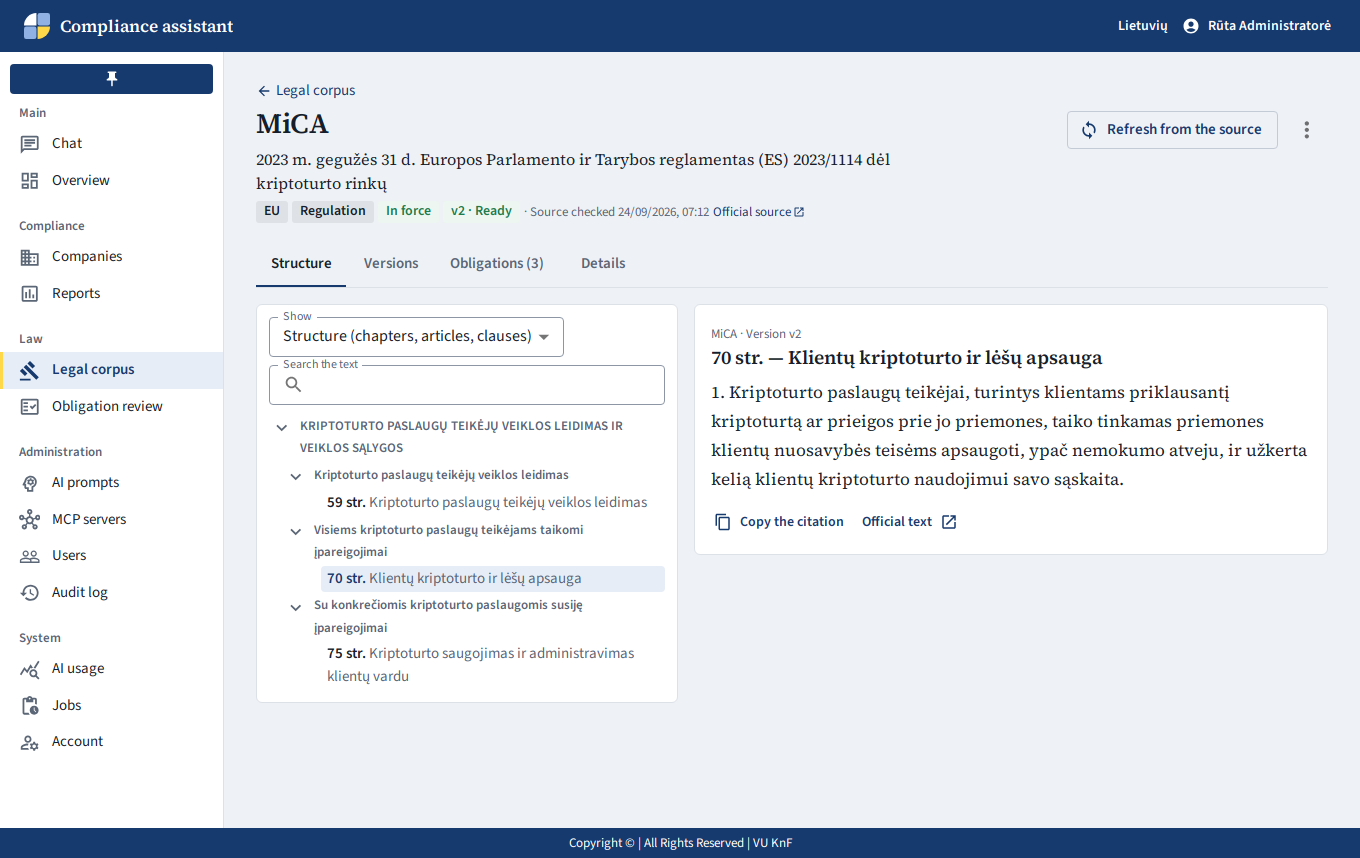
\includegraphics[width=.78\textwidth, trim=240 98 0 52, clip]{figures/screens/corpus-act}
\caption{Vienas teisės aktų bazės aktas, struktūros skiltis: nuostatų medis su filtru ir paieška
ir pasirinkta nuostata šriftu su užraitomis, su \ui{Kopijuoti citatą} ir \ui{Oficialus tekstas}.
Redakcijos žymė ir \ui{Atnaujinti iš šaltinio} (administratoriaus) yra
antraštėje.}\label{fig:console:act}
\end{figure}

Akto puslapis (\file{CorpusDocument.jsx}, \cref{fig:console:act}) turi keturias skiltis:
\ui{Struktūra} (skyrių, straipsnių ir punktų medis šalia pasirinktos nuostatos teksto su jos
oficialia nuoroda), \ui{Redakcijos} (kiekviena išsaugota redakcija su būsena, skaičiais,
struktūros atpažinimo priemone ir vektorizavimo modeliu), \ui{Pareigos} (iš akto išskirtos
pareigos, paprastam naudotojui tik skaitymui) ir \ui{Informacija} (katalogo įrašas, o po jo ---
tai, ką modeliai perskaitė iš paties akto teksto: kam jis taikomas ir kiek sankcijų pakopų
nustato, kiekvienu atveju su modelio palikta pastaba arba užrašu \ui{Dar neskaityta}).
Pasirinkta nuostata yra adrese
(\code{?unit=}), todėl ataskaitos citata gali į ją nurodyti. Administratoriaus veiksmai yra
antraštėje ir jos meniu: \ui{Atnaujinti iš šaltinio}, \ui{Apdoroti iš naujo (net jei
nepasikeitė)}, \ui{Įkelti naują redakciją} (ne daugiau kaip 60~MB), \ui{Išskirti pareigas},
\ui{Patikrinti pareigas} (į eilę įtraukia vertintojo užduotį), \ui{Perskaičiuoti vektorius},
\ui{Redaguoti metaduomenis}, \ui{Įjungti} / \ui{Išjungti} ir \ui{Ištrinti teisės aktą};
standartui dar \ui{Skaityti struktūrą kitaip}. Kiekvienas brangus ar naikinantis veiksmas
pirmiausia patvirtinamas. Paties katalogo antraštėje yra \ui{Pridėti teisės aktą ar standartą},
kurio dialogas prašo šaltinio --- CELEX numerio, e-TAR identifikatoriaus, Lietuvos banko
puslapio, adreso ar įkelto failo --- ir katalogo metaduomenų; jos meniu turi visų šaltinių
patikrą ir visko pervektorizavimą. Mechanizmas aprašytas \cref{ch:corpus}.

\subsection{Pareigų peržiūra}\label{sec:console:obligations}

\begin{figure}[htbp]
\centering
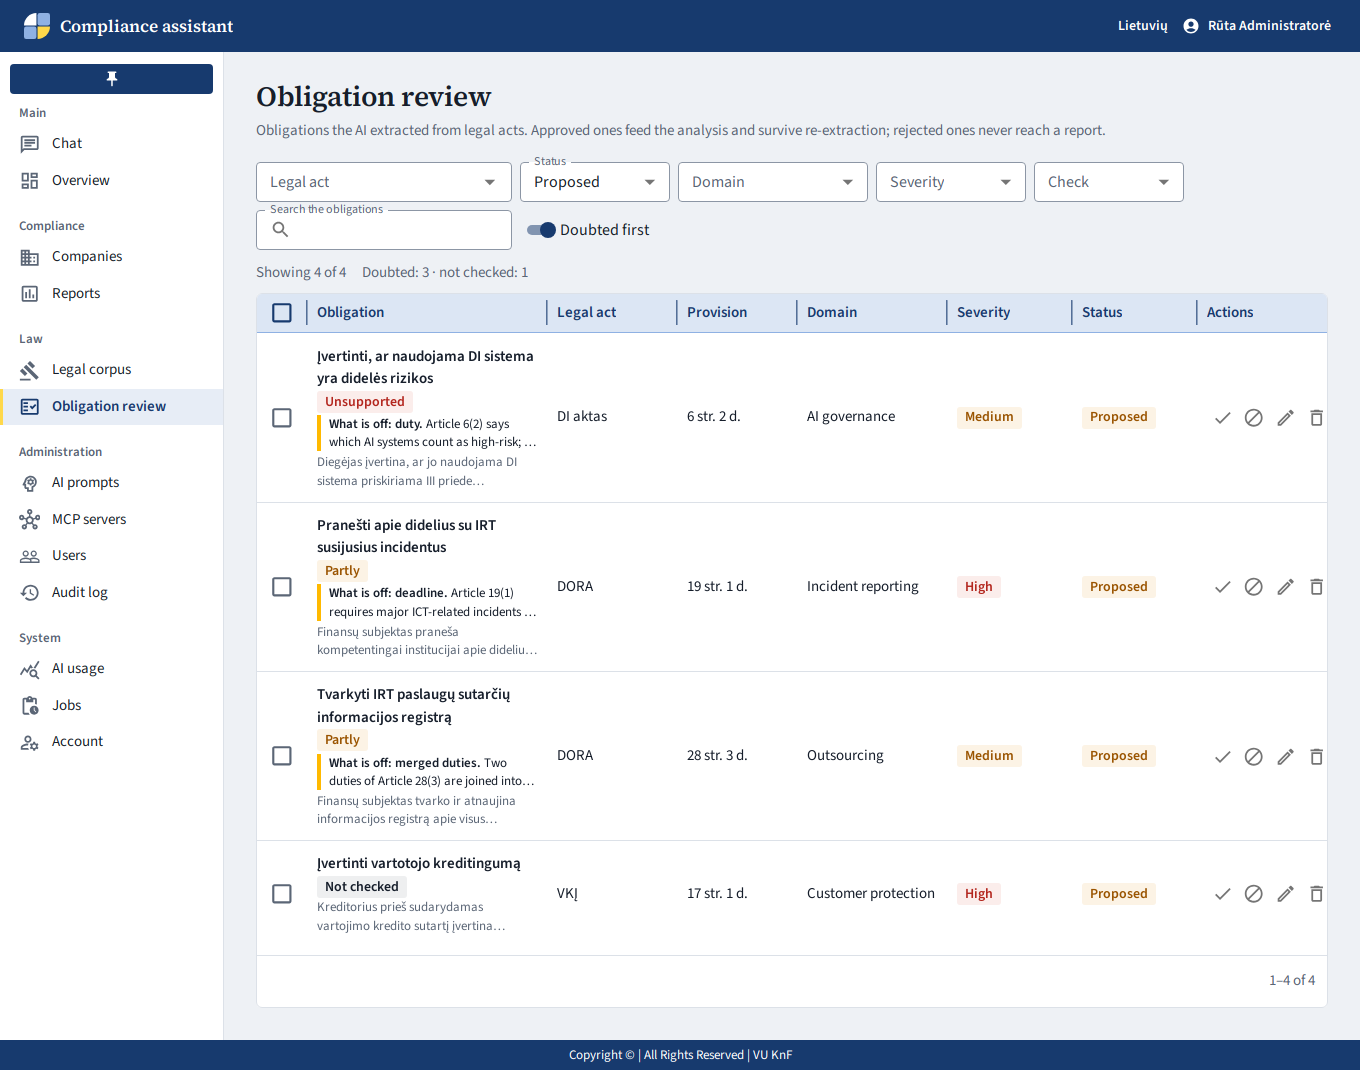
\includegraphics[width=.76\textwidth, trim=240 30 0 52, clip]{figures/screens/obligations}
\caption{Pareigų peržiūra (\code{/console/obligations}) su įjungtu \ui{Abejotinos pirmiausia}. Po
kiekvienu pavadinimu --- vertintojo verdiktas žyme (\ui{Nepagrįsta}, \ui{Iš dalies},
\ui{Netikrinta}) ir, abejotinos pareigos atveju, kas negerai; dešinėje --- eilutės veiksmai:
patvirtinti, atmesti, redaguoti, ištrinti.}\label{fig:console:obligations}
\end{figure}

\ui{Pareigų peržiūra} (\file{pages/Obligations/ObligationsPanel.jsx},
\cref{fig:console:obligations}) yra administratoriaus eilė, kurioje yra kiekviena modelio iš
teisės aktų bazės išskirta pareiga. Ji atsiveria ties pasiūlytomis pareigomis su įjungtu
\ui{Abejotinos pirmiausia}: pareigos, kuriomis suabejojo antrasis modelio iškvietimas,
\term{vertintojas}, palyginęs jas su visu cituojamų nuostatų tekstu, rodomos pirmos, nes nuo jų
pradedama peržiūra. Vertintojo verdiktas yra žymė po pavadinimo --- neryški, kai vertintojas
pareigą pripažino pagrįsta arba jos nevertino, o dėmesį traukiančiais tonais, kai \ui{Iš dalies}
ar \ui{Nepagrįsta}, --- o po abejotina eilute nurodoma, kas negerai, ir vertintojo pastaba.
Vertintojas nieko nesprendžia. Filtrai susiaurina sąrašą pagal aktą, būseną, sritį,
reikšmingumą ir patikrą. Eilutės patvirtinamos, atmetamos ar redaguojamos po vieną arba
pažymimos ir tvarkomos kartu mygtukais \ui{Patvirtinti pažymėtas}, \ui{Atmesti pažymėtas} ar
\ui{Grąžinti į pasiūlytas}; didelis pasirinkimas serveriui siunčiamas po 500. Eilutės pavadinimas
atveria redagavimo dialogą, kuriame virš formos rodomas visas vertintojo verdiktas; pakeitus
pavadinimą ar tekstą, tas verdiktas išvalomas. Tas pats skydelis, tik skaitymui, yra akto pareigų
skiltis paprastam naudotojui. Išskyrimas, vertintojas ir peržiūra aprašyti \cref{ch:obligations}.

\subsection{DI instrukcijos}\label{sec:console:prompts}

\ui{DI instrukcijos} (\file{pages/Prompts/Prompts.jsx}) išvardija kiekvieną išsaugotą pokalbio ir
apdorojimo grandinių instrukciją su aktyvia versija ir modeliu; ženkliukas \ui{Laukia nauja
numatytoji} žymi instrukciją, kuriai diegimas atnešė naujesnę numatytąją versiją, kuri nėra
aktyvi, nes aktyvi yra administratoriaus sukurta versija.

\begin{figure}[htbp]
\centering
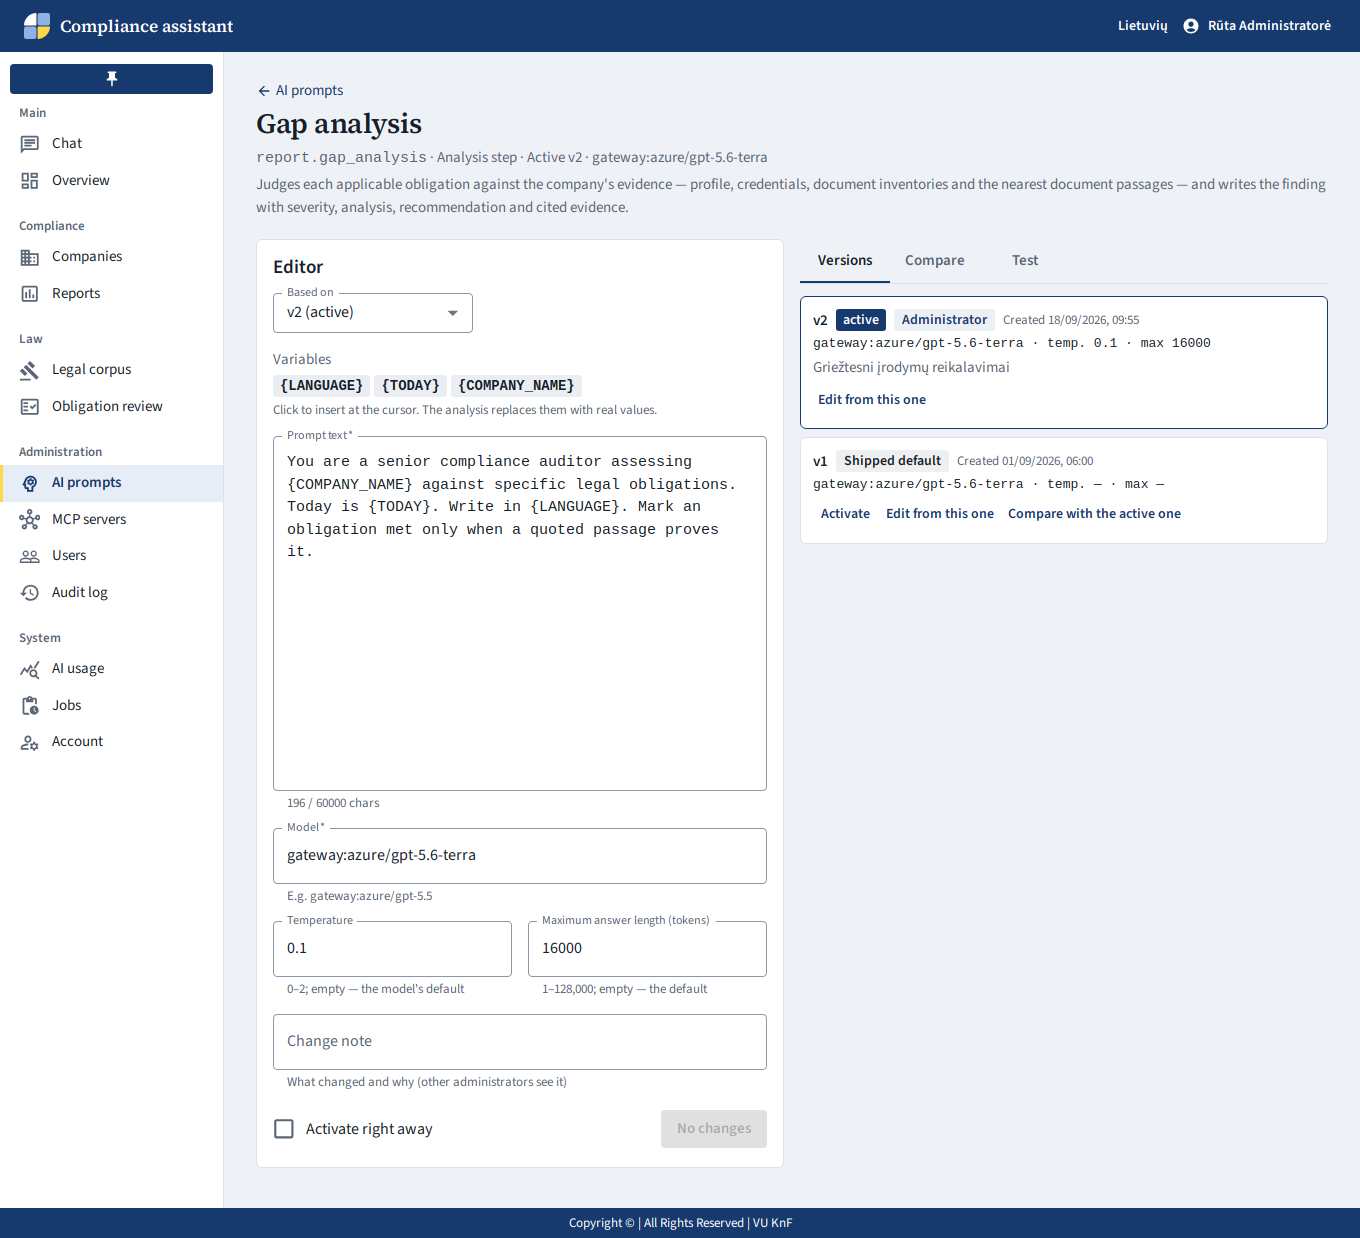
\includegraphics[width=.70\textwidth, trim=240 68 0 52, clip]{figures/screens/prompt-editor}
\caption{Instrukcijų redaktorius. Kairėje --- juodraštis: versija, nuo kurios jis pradėtas,
kintamieji (spustelėjus vienas įterpiamas žymeklio vietoje), tekstas, modelis, temperatūra,
didžiausias atsakymo ilgis, pakeitimo pastaba ir \ui{Iš karto aktyvuoti}. Dešinėje --- skiltys
\ui{Versijos}, \ui{Palyginimas} ir \ui{Bandymas}; istorijoje pažymėta aktyvi versija ir
su diegimu pateikta numatytoji.}\label{fig:console:prompt}
\end{figure}

Redaktorius (\file{PromptEditor.jsx}, \cref{fig:console:prompt}) laiko juodraštį, pradėtą nuo
išsaugotos versijos. Išsaugant versija niekada neperrašoma: pridedama nauja
(\ui{Išsaugoti kaip naują versiją}), o iškart ji aktyvuojama tik tada, kai pažymėta
\ui{Iš karto aktyvuoti}. Šalia juodraščio yra trys skiltys: \ui{Versijos} (patvirtinus
aktyvuoti bet kurią versiją, įkelti ją į redaktorių arba palyginti su aktyvia),
\ui{Palyginimas} (bet kurių dviejų versijų ar juodraščio eilučių skirtumai, o virš teksto
palyginami parametrai) ir \ui{Bandymas} (vienas juodraščio ar versijos vykdymas su modeliu pagal
pateiktą įvestį, rodantis atsakymą, žetonus, kainą ir galutines instrukcijas, kurias gavo
modelis). Bandymas kainuoja pinigus, ir skydelis tai pasako; jis apmokamas iš administratoriaus
biudžeto. Instrukcijų saugykla ir jos taisyklės aprašytos \cref{ch:prompts}.

\subsection{MCP serveriai}\label{sec:console:mcp}

\ui{MCP serveriai} (\file{pages/Mcp/McpServers.jsx}) išvardija išorinių įrankių serverius, kurių
įrankiais gali naudotis pokalbių asistentas, po vieną kortelę: pavadinimas, aprašymas, adresas,
transportas, įjungtas ar išjungtas, jo antraščių pavadinimai (jų reikšmės yra paslaptys ir
niekada negrąžinamos), leidžiami įrankiai ir įrankiai, kuriuos rado paskutinis bandymas. Naujas
serveris sukuriamas išjungtas; \ui{Tikrinti ryšį} prisijungia ir išvardija jo įrankius, kas gali
užtrukti iki maždaug 45 sekundžių, ir tik tada jį galima įjungti. Dialogas tikrina adresą taip
pat, kaip API, --- \code{https} standartiniu prievadu į viešą pavadinimą, jokio IP adreso,
jokio vidinio pavadinimo, jokio naudotojo vardo ir slaptažodžio, --- nes asistentas, kuris prie
jo jungiasi, veikia šalia kiekvienos vidinės paslaugos (\cref{ch:security}). Puslapyje esanti
pastaba primena administratoriui, kad serverio adresą taip pat turi leisti išeinančio srauto
tinklo taisyklės (\cref{ch:ops}).

\subsection{Užduotys}\label{sec:console:jobs}

\ui{Užduotys} (\file{pages/Jobs/Jobs.jsx}) yra eilė: naudotojo užduotys, administratoriui ---
visos, filtruojamos pagal rūšį ir būseną. Eilutės eina darbo tvarka --- pirma vykdomos dabar,
paskui laukiančios ta tvarka, kuria jas paims užduočių vykdytojas, paskui pasibaigusios, --- o
eilutė virš lentelės pasako, kiek vykdoma ir kiek laukia. \ui{Atšaukti užduotį} laukiančią
užduotį atšaukia iškart, o vykdomą sustabdo kitame etape. \ui{Užduoties informacija} atveria
stalčių su užduoties laiko žymomis, bandymais, jos DI sąnaudomis (iškvietimai, žetonai ir
doleriai), klaida, etapais ir rezultatu; kiekvienas baigtas etapas nurodo jį vykdžiusią instrukcijos
versiją (pavyzdžiui, \code{report.summary v3}), savo modelius ir iškvietimus. Užduotys ir
užduočių vykdytojas aprašyti \cref{ch:arch}.

\subsection{DI sąnaudos}\label{sec:console:usage}

\begin{figure}[htbp]
\centering
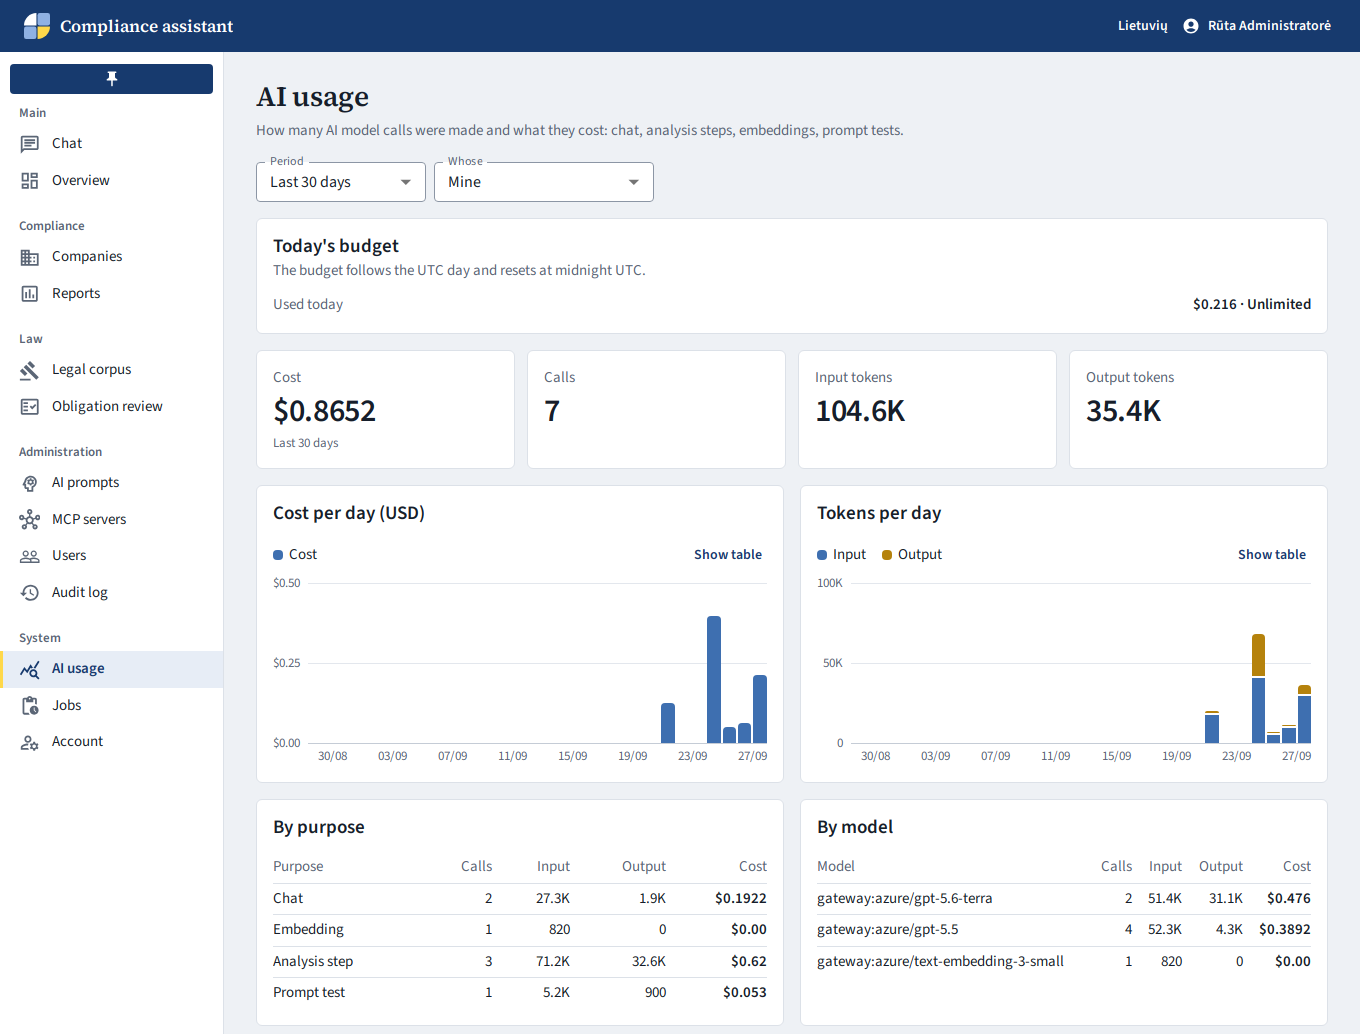
\includegraphics[width=.74\textwidth, trim=240 0 0 52, clip]{figures/screens/usage}
\caption{\ui{DI sąnaudos} vienam naudotojui per 30 dienų: šios dienos biudžetas, laikotarpio
sumos, kaina ir žetonai per dieną dviejose atskirose diagramose ir paskirstymas pagal paskirtį ir
pagal modelį. Po paskirstymais eina iškvietimų žurnalas.}\label{fig:console:usage}
\end{figure}

\ui{DI sąnaudos} (\file{pages/Usage/Usage.jsx}, \cref{fig:console:usage}) rodo, kiek kainavo
modeliai. Pirmiausia rodomas šios dienos biudžetas kaip matuoklis (biudžetas skaičiuojamas pagal
UTC parą), paskui pasirinkto laikotarpio sumos (7, 30 ar 90 dienų: kaina, iškvietimai, įvesties
ir išvesties žetonai), kaina per dieną ir žetonai per dieną dviejose stulpelinėse diagramose ---
du matai, dvi diagramos, niekada ne dvi ašys, --- ir paskirstymas pagal paskirtį (\ui{Pokalbis},
\ui{Analizės etapas}, \ui{Vektorizavimas}, \ui{Instrukcijos bandymas}), pagal modelį ir, kai
administratorius žiūri į visus, pagal naudotoją. \ui{Iškvietimų žurnalas} išvardija kiekvieną
iškvietimą; atvertas jis rodo savo įrankių iškvietimus, o pokalbio ėjimo atveju --- ir
stenogramą: klausimą ir atsakymą. Kiekvienas naudotojas mato savo sąnaudas; administratorius gali
išplėsti vaizdą iki visų paskyrų arba žiūrėti į vieną, todėl čia gali perskaityti kiekvieno
naudotojo pokalbių stenogramas. Tai naudotojams pasakyta naudotojo vadove ir viešojoje svetainėje
ir yra \cref{ch:security} tema; DI sąnaudų žurnalas ir biudžetai aprašyti \cref{ch:models}.

\subsection{Veiksmų žurnalas, naudotojai ir paskyra}\label{sec:console:admin}

\ui{Veiksmų žurnalas} (\file{pages/Audit/Audit.jsx}) išvardija, kas ką ir kada pakeitė,
naujausius įrašus pirmiausia, filtruojant pagal veiksmą (pagal sritį --- prisijungimas,
naudotojai, įmonės, dokumentai, teisės aktai, pareigos, ataskaitos, instrukcijos, MCP serveriai,
užduotys --- arba vieną veiksmą), pagal naudotoją ir pagal momentą \ui{Iki (imtinai)};
\ui{Įkelti senesnius} puslapiais grįžta atgal per įrašų seką. Įrašas atsiveria su savo detalėmis.

\ui{Naudotojai} (\file{pages/Users/Users.jsx}) yra administratoriaus naudotojų sąrašas:
\ui{Naujas naudotojas} su vardu, el. paštu, role (\ui{Administratorius} arba \ui{Naudotojas}) ir
pradiniu ne trumpesniu nei 10 simbolių slaptažodžiu; redaguojami vardas, rolė, paskyros
aktyvumas ir \ui{Dienos DI biudžetas}, kuris yra \ui{Numatytasis} (diegimo nustatytas),
\ui{Neribotas} arba \ui{Individualus} (JAV doleriais per UTC parą); \ui{Keisti slaptažodį}, kuris
baigia to naudotojo sesijas; \ui{Deaktyvuoti}. \ui{Ištrinti su visais duomenimis} neturi
dialogo: mygtuką reikia laikyti nuspaustą dvi sekundes (\file{components/LongPressButton/}), ir
jis ištrina paskyrą su jos įmonėmis, ataskaitomis, dokumentais ir pokalbiais. Administratorius
negali pakeisti savo rolės ar būsenos ir negali ištrinti savęs, o paskutinio aktyvaus administratoriaus
negalima pažeminti ar deaktyvuoti; valdikliai tai pasako dar prieš API atsisakymą.

\ui{Paskyra} (\file{pages/Account/Account.jsx}) rodo naudotojo vardą, el. paštą ir rolę, leidžia
pakeisti slaptažodį (bent 10 simbolių ir ne daugiau kaip 72 baitai; pakeitimas baigia kitas
sesijas) ir siūlo \ui{Atsijungti visuose įrenginiuose}.

\subsection{Valdikliai, kurie pradeda modelio iškvietimą}\label{sec:console:modelbuttons}

\begin{table}[H]
\caption{Konsolės valdikliai, dėl kurių sistema iškviečia modelį, su skyriumi, kuriame yra
iškvietimo kelio kortelė ir kuris pasako, kas moka.}\label{tab:console:modelbuttons}
\begin{tabularx}{\textwidth}{@{}L{40mm}YL{28mm}@{}}
\toprule
\hd{Kur} & \hd{Valdiklis} & \hd{Kelio kortelė} \\
\midrule
Pokalbis & žinutės siuntimas; atsakymo generavimas iš naujo; pirmoji žinutė dar ir suteikia
pokalbiui pavadinimą & \cref{ch:chat} \\
Pradžios dialogas, apimties ekranas & \ui{Pradėti analizę}; \ui{Patvirtinti ir tęsti} &
\cref{ch:report,ch:obligations} \\
Įmonės dokumentai & įkėlimas (indekso vektoriai); paieška dokumentuose (užklausos
vektorius) & \cref{ch:company} \\
Programos skiltis & \ui{Generuoti} / \ui{Generuoti naują versiją} & \cref{ch:programme} \\
Teisės aktų bazė & \ui{Paieška} (užklausos vektorius); \ui{Citatų tikrinimas} su tema &
\cref{ch:corpus,ch:company} \\
Vienas aktas (administratorius) & \ui{Išskirti pareigas}; \ui{Patikrinti pareigas}
(vertintojas); \ui{Perskaičiuoti vektorius}; \ui{Atnaujinti iš šaltinio} arba \ui{Įkelti naują
redakciją} (naujos redakcijos vektoriai; standartui --- dar ir modelis, kuris skaito jo
struktūrą) & \cref{ch:corpus,ch:obligations} \\
Instrukcijų redaktorius (administratorius) & \ui{Paleisti bandymą} & \cref{ch:prompts} \\
\bottomrule
\end{tabularx}
\end{table}

% ------------------------------------------------------------
\section{Kur sprendžia žmogus}\label{sec:console:decisions}

Sistema tam tikrus sprendimus palieka žmogui ir niekada jų nepriima pati. Kiekvienas turi vieną
vietą konsolėje ir vieną valdiklį. \Cref{tab:console:decisions} juos surenka; nurodyti skyriai
paaiškina, ką kiekvienas sprendimas keičia.

\begin{xltabular}{\textwidth}{@{}L{30mm}L{34mm}YL{18mm}@{}}
\caption{Sprendimai, kuriuos konsolė palieka žmogui, puslapis, kuriame yra kiekvienas, ir
valdiklis.}\label{tab:console:decisions}\\
\toprule
\hd{Sprendimas} & \hd{Puslapis} & \hd{Valdiklis ir ką jis užrašo} & \hd{Skyrius} \\
\midrule
\endfirsthead
\toprule
\hd{Sprendimas} & \hd{Puslapis} & \hd{Valdiklis ir ką jis užrašo} & \hd{Skyrius} \\
\midrule
\endhead
\bottomrule
\endlastfoot
Pradėti brangią analizę & Pradžios dialogas (įmonės puslapis, ataskaitų puslapis) &
\ui{Pradėti analizę}, parodžius viršutinės ribos įvertį ir likusį biudžetą. Pokalbyje
asistentas parodo įvertį ir pradeda tik tada, kai naudotojas aiškiai sutinka. &
\cref{ch:report,ch:chat} \\
Patvirtinti ataskaitos apimtį & Laukianti ataskaita, skiltis \ui{Teisės aktai} & Jungiklis
\ui{Vertinti} kiekvienam aktui, paskui \ui{Patvirtinti ir tęsti}; arba \ui{Atšaukti analizę}.
Ataskaita užrašo, kas ir kada patvirtino sąrašą, ir aktus, dėl kurių nuspręsta priešingai
verdiktui. Pokalbyje asistentas parodo sąrašą ir kainą ir tęsia tik naudotojui sutikus. &
\cref{ch:report,ch:chat} \\
Patvirtinti pareigą & \ui{Pareigų peržiūra}; redagavimo dialogas & Eilutės patvirtinimo ar
atmetimo piktograma arba \ui{Patvirtinti pažymėtas} / \ui{Atmesti pažymėtas} / \ui{Grąžinti į
pasiūlytas} pasirinktoms; pakeitimai dialoge. Vertintojo verdiktas parodomas ir nieko
nesprendžia. & \cref{ch:obligations} \\
Pakeisti išvados būseną, užrašyti jos priežastį & Baigta ataskaita, skiltis \ui{Išvados} &
\ui{Peržiūrėti} atveria dialogą: palikti DI vertinimą arba pasirinkti būseną, pastaba,
\ui{Priežastis}. Pažymima \ui{Peržiūrėta}; atšaukia patvirtinimą. & \cref{ch:report} \\
Patvirtinti ataskaitą & Baigta ataskaita, antraštė & \ui{Patvirtinti ataskaitą} su neprivaloma
pastaba; \ui{Atšaukti patvirtinimą} jį atšaukia. Užrašo, kas ir kada, ir pajudina veiksmų
registrą. & \cref{ch:register} \\
Prižiūrėti veiksmą, uždaryti jį rankiniu būdu & Įmonės skiltis \ui{Veiksmai}, atverta eilutė &
Atsakingas asmuo, terminas, būsena, pastaba; uždarant rankiniu būdu reikia pastabos, kuri
užrašo kodėl. & \cref{ch:register} \\
Patikrinti leidimą & Įmonės skiltis \ui{Leidimai ir licencijos} & \ui{Pažymėti patikrintu},
patvirtinus; užrašo, kas ir kada. Atitikties spragų analizei nurodoma, kad deklaruota licencija
yra įmonės žodis: ji gali pagrįsti \status{met} tik su išlyga, kad ją reikia patikrinti.
Pokalbyje asistentas leidimą pažymi patikrintu tik naudotojui aiškiai pasakius, kad jis buvo
patikrintas. &
\cref{ch:company,ch:chat} \\
Patvirtinti programos dokumentą & Programos dokumento puslapis, antraštė & \ui{Patvirtinti},
išjungtas, kol pažeista blokuojanti taisyklė ar yra neišsaugotų pakeitimų; neprivaloma pastaba.
Užrašo, kas ir kada; užfiksuoja dokumentą. & \cref{ch:programme} \\
Aktyvuoti instrukcijos versiją & Instrukcijų redaktorius & \ui{Aktyvuoti} ties versija
(patvirtinus), \ui{Iš karto aktyvuoti} išsaugant arba \ui{Aktyvuoti} ties laukiančia su diegimu
pateikta numatytąja versija. & \cref{ch:prompts} \\
\end{xltabular}

\begin{humanbox}{Ko konsolė niekada nedaro vietoj žmogaus}
Joks konsolės valdiklis nieko nepatvirtina (nei pavienio įrašo, nei ataskaitos) ir neaktyvuoja,
jei jo nepaspaudžia žmogus, o vietos, kuriose modelio rezultatas patenka į įrašus, taip ir
pažymėtos: išvada, kurios būseną pakeitė žmogus, rodo \ui{Peržiūrėta}, o modelio verdiktą
išsaugo iššokančiame paaiškinime; išvada,
kurios pareigos nepatvirtino joks žmogus, rodo \ui{Nepatvirtinta pareiga}; be apimties peržiūros
vykdyta ataskaita rodo \ui{Ataskaita paleista be aktų sąrašo peržiūros}. Spragos priežasties
nerašo joks modelis.
\end{humanbox}

% ------------------------------------------------------------
\section{Viešoji svetainė}\label{sec:console:site}

\begin{figure}[htbp]
\centering

\includegraphics[width=.70\textwidth]{figures/screens/site-home}
\caption{Pirmasis viešosios svetainės puslapis. Tamsi juosta yra konsolės: žodinis ženklas,
keturi puslapiai, kalbos jungiklis ir kelias į konsolę --- čia \ui{Atverti konsolę}, nes ši
naršyklė turi sesiją; lankytojas be jos mato \ui{Prisijungti}. Pagrindiniame bloke ženklas
parodytas kaip trimatis objektas.}\label{fig:console:site}
\end{figure}

Viešoji svetainė (\file{site/}, \cref{fig:console:site}) yra penki puslapiai po ta pačia tamsia
juosta kaip konsolėje (\file{site/router.jsx}). Tai paprasta React programa su bendru stilių failu, be
komponentų bibliotekos. Kelias į konsolę jos juostoje vadinasi \ui{Prisijungti} arba
\ui{Atverti konsolę}, kai naršyklė jau turi sesijos prieigos raktą (\file{site/parts.jsx}). Tai,
ką puslapiai sako apie analizę ir duomenis, atitinka naudotojo vadovą
(\file{docs/markdown/lt/user-guide.md}), o README prašo abu keisti kartu.

\begin{table}[H]
\caption{Viešosios svetainės puslapiai.}\label{tab:console:sitepages}
\begin{tabularx}{\textwidth}{@{}L{34mm}Y@{}}
\toprule
\hd{Puslapis} & \hd{Ką jis sako} \\
\midrule
\code{/} \ui{Atitikties spragų analizė finansų įstaigoms} & Teiginys \enquote{Atitiktis yra
mozaika. Parodome, kurių detalių trūksta.}; viena išvada iš arti su ją lemiančia, pažymėta įmonės
dokumento ištrauka; trys dalykai, kuriuos daro asistentas (nustato, kurie aktai taikomi, tikrina
kiekvieną pareigą pagal dokumentus, sudaro veiksmų planą); ataskaita; pokalbis; iš kur imami
tekstai (ES leidinių biuras, e-TAR, Lietuvos bankas); ir ko asistentas nedaro. \\
\code{/product} \ui{Produktas} & Kelias nuo pokalbio iki patvirtintos ataskaitos, žingsnis po
žingsnio: pokalbis, analizė su iš anksto žinoma kaina, išvada su įrodymais, veiksmų planas,
pačių dokumentų nuorodų patikra, peržiūra, patvirtinimas ir eksportas. \\
\code{/method} \ui{Metodika} & Šeši analizės žingsniai; ką ataskaita daro su aktu priklausomai
nuo to, kaip jis taikomas; penkios būsenos ir ką reiškia reikšmingumas; kas lieka žmogui
(peržiūra, patvirtinimas, kilmė); ko asistentas nedaro. \\
\code{/sources} \ui{Teisės aktai} & Kaip saugomi tekstai (suskaidyti iki punkto, tikrinami kas
savaitę, susieti su oficialiu tekstu) ir teisės aktų bazės aktai pagal kilmę --- ES aktai, Lietuvos
įstatymai, priežiūros institucijų aktai, --- paskui licencijavimo puslapiai ir standartai; sąrašas
nurodo, kad tai teisės aktų bazė 2026 m. lapkričio mėn. būklės (\file{site/acts.js}, rankiniu būdu
derinama su katalogu). \\
\code{/about} \ui{Apie} & Kur ir kuriam kursui produktas sukurtas, kam jis skirtas, kaip
suteikiama prieiga (paskyras kuria administratorius), kas vyksta su naudotojo duomenimis, kaip
jis sukurtas, ir perspėjimas, kad jo išvados yra pagalbinė priemonė. \\
\bottomrule
\end{tabularx}
\end{table}

Svetainė rodo patį produktą, o ne jo paveikslėlius: \file{site/specimens.jsx} perpiešia nedideles
konsolės ekranų dalis --- išvadą su įrodymais, būsenų juostą, veiksmų planą, pirmąjį ataskaitos
puslapį, pokalbį, nuorodų patikrą, dirbančią analizę --- kaip tikrą tekstą lankytojo kalba, su
išgalvotu turiniu ir pačios konsolės etiketėmis, todėl svetainė negali pavadinti būsenos kitaip
nei produktas. Pagrindinis ir metodikos puslapiai baigiasi tomis pačiomis trimis ribomis
(\file{site/Limits.jsx}): asistentas nepakeičia teisininko, nevertina praktikos ir nespėlioja.
Skaitant puslapius jų dalys juda; kai naršyklėje įjungtas sumažinto judesio nustatymas, dalys
iškart rodomos savo galutinėje vietoje. Svetainės \file{robots.txt} vis dar neleidžia paieškos sistemoms
indeksuoti viso šaltinio.

% ------------------------------------------------------------
\section{Kaip sukurta konsolė}\label{sec:console:built}

\paragraph{Bibliotekos.} Konsolė yra React~19 programa, sukurta su Vite~7. Jos komponentai yra
MUI~7 (lentelėms --- MUI~X duomenų tinklelis), stilizuoti kartu su Tailwind~4; pokalbis sukurtas
su assistant-ui ir AI SDK transportu. Maršrutizavimas --- React Router~7, maršrutai faile
\file{router.jsx} po baze \code{/console}, o kiekvienas puslapis yra modulis, įkeliamas pirmą
kartą jį aplankius. Duomenys gaunami su axios per vieną klientą ir laikomi TanStack Query podėlyje
(\cref{sec:console:data}). Versijos yra tos, kurios nurodytos \file{vite/app/package.json}.
Gamybinis atvaizdas sukuria failus ir pateikia juos kaip statinius failus; atvaizdavimo serverio
pusėje nėra.

\paragraph{Bendros dalys.} Puslapius vienodus išlaiko viena duomenų lentelė
(\file{components/DataTable/DataTable.jsx}), vienas dialogo langas
(\file{components/UniversalModal/UniversalModal.jsx}), viena būsenos žymė, kurios žodžiai neša
būseną, o spalva ją tik pakartoja (\file{components/StatusChip/StatusChip.jsx}), ir viena
numetimo zona, kuri dar prieš siųsdama atmeta neperskaitomą ar per didelį failą
(\file{components/FileDrop/FileDrop.jsx}).

\paragraph{Dvi kalbos, išlaikomos suderintos.} Žodžiai gyvena kataloge \file{messages/}: po vieną
lietuvišką ir vieną anglišką failą kiekvienam puslapiui, komponentui ir etikečių rinkiniui;
\file{i18n.jsx} suranda raktą, o trūkstamas raktas ekrane parodytų savo pavadinimą su taškais,
nes vykdymo metu grįžtama iš vienos kalbos į kitą tik visa apimtimi, niekada ne rakto lygmeniu.
Sargas, \file{vite/app/scripts/check-messages.js}, paleidžiamas prieš kiekvieną stiliaus patikrą
(\en{lint}) ir kiekvieną surinkimą ir baigiasi klaida, jei raktas yra vienoje kalboje, bet nėra
kitoje, jei kintamieji abiejose kalbose skiriasi, jei angliška eilutė sutampa su lietuviška
(neišversta eilutė) ir jei kode yra pažodinis raktas, kuris niekur neveda. 2026 m. lapkričio
13 d. jis suskaičiavo po 2\,824 raktus kiekvienoje kalboje ir patikrino 2\,093 vertimo
iškvietimus.

\paragraph{Išvaizda.} Viena šviesi tema (\file{theme.js}), sukurta iš prekės ženklo lentelės.
Spalvos yra keturių plytelių ženklo spalvos: rašalo mėlyna (\texttt{\#173A6E}) --- viršutinei juostai,
mygtukams, nuorodoms ir fokuso žiedui; vidurinė ženklo mėlyna (\texttt{\#3E6FB0}) --- dabartinės
vietos atspalviui ir eigai; ir jo geltona (\texttt{\#FFD84A}) --- kaip žymeklis: cituojamų
įrodymų ir teksto pažymėjimo paryškinimas bei dabartinio puslapio juostelė navigacijoje. Geltona
niekada neužpildo valdiklio ir ant jos nerašomas tekstas. Balti lapai su labai plonomis kraštinėmis guli
ant pilkai mėlyno fono; šešėlį meta tik plaukiojantys sluoksniai; būsenų spalvos skirtos
verdiktams ir būsenoms ir visada lydimos etiketės. Du šriftai, talpinami pačių: Source Sans~3
sąsajai ir asistento atsakymams, Source Serif~4 puslapių pavadinimams ir visam tam, kas cituojama
iš šaltinio, --- nuostatoms, pareigoms, įmonės dokumentų ištraukoms, --- todėl skaitytojas visada
gali atskirti šaltinį nuo komentaro apie jį. Visur didžiąja raide rašomas tik pirmasis žodis. Šiais šriftais ir spalvomis surinktas ir šis dokumentas.

\paragraph{Testai.} Kiekvienas puslapis, komponentas ir kabliukas (\en{hook}) testuojamas su
vitest imituotoje naršyklėje prieš procese veikiantį serverio pusės dublerį, kuris atsako į
kiekvieną konsolės kviečiamą galinį tašką; užklausa, į kurią neatsako joks apdorojimo
komponentas, sužlugdo savo testą, o kiekvienas puslapis testuojamas su abiem rolėmis ir abiem
kalbomis. Testų rinkiniai ir jų skaičiai aprašyti \cref{ch:testing}.
